%-*-latex-*-
\tinysidebar{\debug{exercises/20-n5-n3-1-5n3-cos-n-7-8/answer.tex}}
(a)
Let $f_0(n) = 20 n^5/(n^3 + 1)$.
The following is a plot of $|f_0(n)|$ and $20n^2$:
%-*-latex-*-

\begin{center}
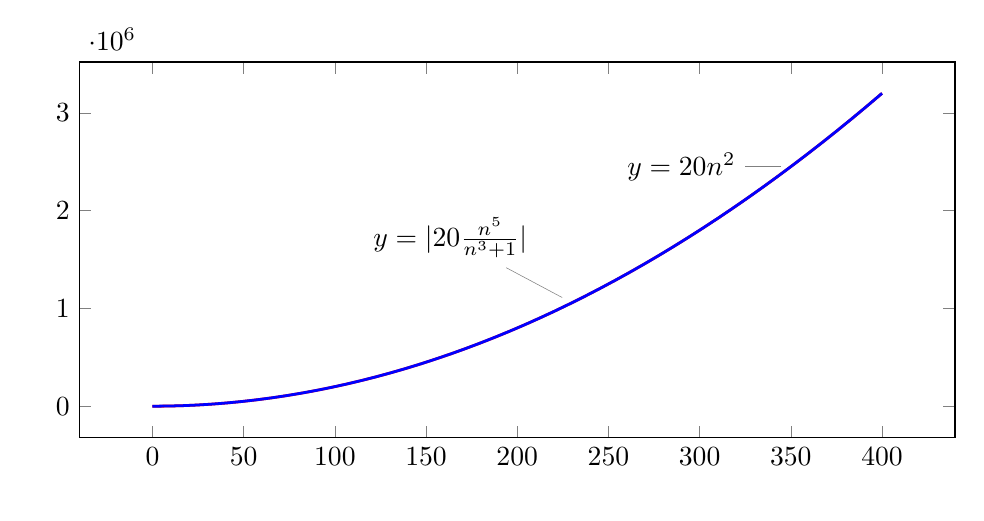
\begin{tikzpicture}[line width=1]
\begin{axis}[width=5in, height=2.5in,
             scatter/classes={a={mark=*,draw=black}},
             xlabel={\mbox{}},
             xlabel style={name=xlabel}, 
             ylabel={\mbox{}}, 
             legend style={
                at={(xlabel.south)},
                yshift=-1ex,
                anchor=north,
                legend cell align=left,
                },
        ]
]
\addplot[draw=red, line width=1] coordinates {(0.0,0.0)
(0.4004,0.1934)
(0.8008,4.3517)
(1.2012,18.2995)
(1.6016,41.2596)
(2.002,71.2773)
(2.4024,107.6658)
(2.8028,150.2884)
(3.2032,199.1508)
(3.6036,254.2853)
(4.004,315.7226)
(4.4044,383.4872)
(4.8048,457.5977)
(5.2052,538.068)
(5.6056,624.9086)
(6.006,718.1275)
(6.4064,817.7308)
(6.8068,923.7234)
(7.2072,1036.1091)
(7.6076,1154.8909)
(8.008,1280.0712)
(8.4084,1411.6521)
(8.8088,1549.6351)
(9.2092,1694.0217)
(9.6096,1844.813)
(10.01,2002.01)
(10.4104,2165.6134)
(10.8108,2335.6241)
(11.2112,2512.0425)
(11.6116,2694.8692)
(12.012,2884.1046)
(12.4124,3079.7492)
(12.8128,3281.8032)
(13.2132,3490.2671)
(13.6136,3705.141)
(14.014,3926.4252)
(14.4144,4154.1198)
(14.8148,4388.2252)
(15.2152,4628.7414)
(15.6156,4875.6686)
(16.016,5129.0069)
(16.4164,5388.7565)
(16.8168,5654.9175)
(17.2172,5927.49)
(17.6176,6206.474)
(18.018,6491.8697)
(18.4184,6783.677)
(18.8188,7081.8962)
(19.2192,7386.5273)
(19.6196,7697.5702)
(20.02,8015.0252)
(20.4204,8338.8921)
(20.8208,8669.1711)
(21.2212,9005.8622)
(21.6216,9348.9655)
(22.022,9698.481)
(22.4224,10054.4087)
(22.8228,10416.7486)
(23.2232,10785.5008)
(23.6236,11160.6653)
(24.024,11542.2422)
(24.4244,11930.2314)
(24.8248,12324.633)
(25.2252,12725.4469)
(25.6256,13132.6734)
(26.026,13546.3122)
(26.4264,13966.3635)
(26.8268,14392.8273)
(27.2272,14825.7035)
(27.6276,15264.9923)
(28.028,15710.6936)
(28.4284,16162.8074)
(28.8288,16621.3337)
(29.2292,17086.2726)
(29.6296,17557.6241)
(30.03,18035.3881)
(30.4304,18519.5647)
(30.8308,19010.1539)
(31.2312,19507.1557)
(31.6316,20010.5701)
(32.032,20520.3972)
(32.4324,21036.6368)
(32.8328,21559.2891)
(33.2332,22088.354)
(33.6336,22623.8316)
(34.034,23165.7218)
(34.4344,23714.0247)
(34.8348,24268.7402)
(35.2352,24829.8684)
(35.6356,25397.4093)
(36.036,25971.3629)
(36.4364,26551.7291)
(36.8368,27138.508)
(37.2372,27731.6997)
(37.6376,28331.304)
(38.038,28937.321)
(38.4384,29549.7507)
(38.8388,30168.5931)
(39.2392,30793.8482)
(39.6396,31425.5161)
(40.04,32063.5966)
(40.4404,32708.0899)
(40.8408,33358.9959)
(41.2412,34016.3146)
(41.6416,34680.0461)
(42.042,35350.1903)
(42.4424,36026.7472)
(42.8428,36709.7168)
(43.2432,37399.0992)
(43.6436,38094.8944)
(44.044,38797.1022)
(44.4444,39505.7228)
(44.8448,40220.7562)
(45.2452,40942.2023)
(45.6456,41670.0612)
(46.046,42404.3328)
(46.4464,43145.0172)
(46.8468,43892.1143)
(47.2472,44645.6241)
(47.6476,45405.5468)
(48.048,46171.8822)
(48.4484,46944.6303)
(48.8488,47723.7913)
(49.2492,48509.3649)
(49.6496,49301.3514)
(50.0501,50099.7506)
(50.4505,50904.5626)
(50.8509,51715.7873)
(51.2513,52533.4249)
(51.6517,53357.4752)
(52.0521,54187.9382)
(52.4525,55024.8141)
(52.8529,55868.1027)
(53.2533,56717.8041)
(53.6537,57573.9182)
(54.0541,58436.4452)
(54.4545,59305.3849)
(54.8549,60180.7374)
(55.2553,61062.5027)
(55.6557,61950.6808)
(56.0561,62845.2716)
(56.4565,63746.2753)
(56.8569,64653.6917)
(57.2573,65567.5209)
(57.6577,66487.7629)
(58.0581,67414.4176)
(58.4585,68347.4852)
(58.8589,69286.9655)
(59.2593,70232.8587)
(59.6597,71185.1646)
(60.0601,72143.8833)
(60.4605,73109.0148)
(60.8609,74080.5591)
(61.2613,75058.5162)
(61.6617,76042.886)
(62.0621,77033.6687)
(62.4625,78030.8641)
(62.8629,79034.4724)
(63.2633,80044.4934)
(63.6637,81060.9273)
(64.0641,82083.7739)
(64.4645,83113.0333)
(64.8649,84148.7055)
(65.2653,85190.7906)
(65.6657,86239.2884)
(66.0661,87294.199)
(66.4665,88355.5224)
(66.8669,89423.2586)
(67.2673,90497.4076)
(67.6677,91577.9694)
(68.0681,92664.944)
(68.4685,93758.3314)
(68.8689,94858.1316)
(69.2693,95964.3446)
(69.6697,97076.9704)
(70.0701,98196.009)
(70.4705,99321.4604)
(70.8709,100453.3246)
(71.2713,101591.6016)
(71.6717,102736.2914)
(72.0721,103887.394)
(72.4725,105044.9094)
(72.8729,106208.8376)
(73.2733,107379.1786)
(73.6737,108555.9324)
(74.0741,109739.099)
(74.4745,110928.6784)
(74.8749,112124.6706)
(75.2753,113327.0757)
(75.6757,114535.8935)
(76.0761,115751.1241)
(76.4765,116972.7676)
(76.8769,118200.8238)
(77.2773,119435.2929)
(77.6777,120676.1747)
(78.0781,121923.4694)
(78.4785,123177.1768)
(78.8789,124437.2971)
(79.2793,125703.8302)
(79.6797,126976.7761)
(80.0801,128256.1348)
(80.4805,129541.9063)
(80.8809,130834.0906)
(81.2813,132132.6877)
(81.6817,133437.6976)
(82.0821,134749.1203)
(82.4825,136066.9559)
(82.8829,137391.2042)
(83.2833,138721.8653)
(83.6837,140058.9393)
(84.0841,141402.4261)
(84.4845,142752.3256)
(84.8849,144108.638)
(85.2853,145471.3632)
(85.6857,146840.5012)
(86.0861,148216.052)
(86.4865,149598.0156)
(86.8869,150986.3921)
(87.2873,152381.1813)
(87.6877,153782.3834)
(88.0881,155189.9982)
(88.4885,156604.0259)
(88.8889,158024.4664)
(89.2893,159451.3196)
(89.6897,160884.5857)
(90.0901,162324.2646)
(90.4905,163770.3564)
(90.8909,165222.8609)
(91.2913,166681.7782)
(91.6917,168147.1084)
(92.0921,169618.8513)
(92.4925,171097.0071)
(92.8929,172581.5757)
(93.2933,174072.5571)
(93.6937,175569.9513)
(94.0941,177073.7583)
(94.4945,178583.9781)
(94.8949,180100.6108)
(95.2953,181623.6562)
(95.6957,183153.1145)
(96.0961,184688.9856)
(96.4965,186231.2695)
(96.8969,187779.9662)
(97.2973,189335.0757)
(97.6977,190896.598)
(98.0981,192464.5331)
(98.4985,194038.8811)
(98.8989,195619.6418)
(99.2993,197206.8154)
(99.6997,198800.4018)
(100.1001,200400.401)
(100.5005,202006.813)
(100.9009,203619.6378)
(101.3013,205238.8755)
(101.7017,206864.5259)
(102.1021,208496.5892)
(102.5025,210135.0653)
(102.9029,211779.9542)
(103.3033,213431.2559)
(103.7037,215088.9704)
(104.1041,216753.0977)
(104.5045,218423.6379)
(104.9049,220100.5908)
(105.3053,221783.9566)
(105.7057,223473.7352)
(106.1061,225169.9266)
(106.5065,226872.5308)
(106.9069,228581.5478)
(107.3073,230296.9777)
(107.7077,232018.8203)
(108.1081,233747.0758)
(108.5085,235481.7441)
(108.9089,237222.8252)
(109.3093,238970.3191)
(109.7097,240724.2258)
(110.1101,242484.5453)
(110.5105,244251.2777)
(110.9109,246024.4229)
(111.3113,247803.9808)
(111.7117,249589.9516)
(112.1121,251382.3353)
(112.5125,253181.1317)
(112.9129,254986.3409)
(113.3133,256797.963)
(113.7137,258615.9979)
(114.1141,260440.4455)
(114.5145,262271.306)
(114.9149,264108.5794)
(115.3153,265952.2655)
(115.7157,267802.3644)
(116.1161,269658.8762)
(116.5165,271521.8008)
(116.9169,273391.1382)
(117.3173,275266.8884)
(117.7177,277149.0514)
(118.1181,279037.6272)
(118.5185,280932.6159)
(118.9189,282834.0174)
(119.3193,284741.8316)
(119.7197,286656.0587)
(120.1201,288576.6987)
(120.5205,290503.7514)
(120.9209,292437.2169)
(121.3213,294377.0953)
(121.7217,296323.3865)
(122.1221,298276.0905)
(122.5225,300235.2073)
(122.9229,302200.7369)
(123.3233,304172.6793)
(123.7237,306151.0346)
(124.1241,308135.8027)
(124.5245,310126.9836)
(124.9249,312124.5773)
(125.3253,314128.5838)
(125.7257,316139.0031)
(126.1261,318155.8353)
(126.5265,320179.0802)
(126.9269,322208.738)
(127.3273,324244.8086)
(127.7277,326287.292)
(128.1281,328336.1883)
(128.5285,330391.4973)
(128.9289,332453.2192)
(129.3293,334521.3539)
(129.7297,336595.9013)
(130.1301,338676.8617)
(130.5305,340764.2348)
(130.9309,342858.0207)
(131.3313,344958.2195)
(131.7317,347064.8311)
(132.1321,349177.8555)
(132.5325,351297.2927)
(132.9329,353423.1427)
(133.3333,355555.4056)
(133.7337,357694.0812)
(134.1341,359839.1697)
(134.5345,361990.671)
(134.9349,364148.5851)
(135.3353,366312.912)
(135.7357,368483.6518)
(136.1361,370660.8043)
(136.5365,372844.3697)
(136.9369,375034.3479)
(137.3373,377230.7389)
(137.7377,379433.5427)
(138.1381,381642.7594)
(138.5385,383858.3888)
(138.9389,386080.4311)
(139.3393,388308.8862)
(139.7397,390543.7541)
(140.1401,392785.0349)
(140.5405,395032.7284)
(140.9409,397286.8348)
(141.3413,399547.3539)
(141.7417,401814.2859)
(142.1421,404087.6308)
(142.5425,406367.3884)
(142.9429,408653.5588)
(143.3433,410946.1421)
(143.7437,413245.1382)
(144.1441,415550.5471)
(144.5445,417862.3688)
(144.9449,420180.6033)
(145.3453,422505.2507)
(145.7457,424836.3108)
(146.1461,427173.7838)
(146.5465,429517.6696)
(146.9469,431867.9682)
(147.3473,434224.6797)
(147.7477,436587.8039)
(148.1481,438957.341)
(148.5485,441333.2909)
(148.9489,443715.6536)
(149.3493,446104.4291)
(149.7497,448499.6174)
(150.1502,450901.2186)
(150.5506,453309.2326)
(150.951,455723.6594)
(151.3514,458144.499)
(151.7518,460571.7514)
(152.1522,463005.4166)
(152.5526,465445.4947)
(152.953,467891.9856)
(153.3534,470344.8893)
(153.7538,472804.2058)
(154.1542,475269.9351)
(154.5546,477742.0773)
(154.955,480220.6322)
(155.3554,482705.6)
(155.7558,485196.9806)
(156.1562,487694.774)
(156.5566,490198.9803)
(156.957,492709.5993)
(157.3574,495226.6312)
(157.7578,497750.0759)
(158.1582,500279.9334)
(158.5586,502816.2037)
(158.959,505358.8868)
(159.3594,507907.9828)
(159.7598,510463.4916)
(160.1602,513025.4132)
(160.5606,515593.7476)
(160.961,518168.4948)
(161.3614,520749.6549)
(161.7618,523337.2277)
(162.1622,525931.2134)
(162.5626,528531.6119)
(162.963,531138.4232)
(163.3634,533751.6474)
(163.7638,536371.2843)
(164.1642,538997.3341)
(164.5646,541629.7967)
(164.965,544268.6721)
(165.3654,546913.9603)
(165.7658,549565.6613)
(166.1662,552223.7752)
(166.5666,554888.3019)
(166.967,557559.2414)
(167.3674,560236.5937)
(167.7678,562920.3588)
(168.1682,565610.5368)
(168.5686,568307.1275)
(168.969,571010.1311)
(169.3694,573719.5475)
(169.7698,576435.3767)
(170.1702,579157.6188)
(170.5706,581886.2736)
(170.971,584621.3413)
(171.3714,587362.8218)
(171.7718,590110.7151)
(172.1722,592865.0212)
(172.5726,595625.7402)
(172.973,598392.872)
(173.3734,601166.4165)
(173.7738,603946.3739)
(174.1742,606732.7442)
(174.5746,609525.5272)
(174.975,612324.723)
(175.3754,615130.3317)
(175.7758,617942.3532)
(176.1762,620760.7875)
(176.5766,623585.6346)
(176.977,626416.8946)
(177.3774,629254.5674)
(177.7778,632098.6529)
(178.1782,634949.1513)
(178.5786,637806.0625)
(178.979,640669.3866)
(179.3794,643539.1234)
(179.7798,646415.2731)
(180.1802,649297.8356)
(180.5806,652186.8109)
(180.981,655082.199)
(181.3814,657984.0)
(181.7818,660892.2137)
(182.1822,663806.8403)
(182.5826,666727.8797)
(182.983,669655.3319)
(183.3834,672589.197)
(183.7838,675529.4748)
(184.1842,678476.1655)
(184.5846,681429.269)
(184.985,684388.7853)
(185.3854,687354.7144)
(185.7858,690327.0563)
(186.1862,693305.8111)
(186.5866,696290.9787)
(186.987,699282.5591)
(187.3874,702280.5523)
(187.7878,705284.9583)
(188.1882,708295.7772)
(188.5886,711313.0089)
(188.989,714336.6534)
(189.3894,717366.7107)
(189.7898,720403.1808)
(190.1902,723446.0637)
(190.5906,726495.3595)
(190.991,729551.0681)
(191.3914,732613.1895)
(191.7918,735681.7237)
(192.1922,738756.6707)
(192.5926,741838.0306)
(192.993,744925.8033)
(193.3934,748019.9887)
(193.7938,751120.5871)
(194.1942,754227.5982)
(194.5946,757341.0221)
(194.995,760460.8589)
(195.3954,763587.1085)
(195.7958,766719.7709)
(196.1962,769858.8461)
(196.5966,773004.3341)
(196.997,776156.235)
(197.3974,779314.5487)
(197.7978,782479.2752)
(198.1982,785650.4145)
(198.5986,788827.9666)
(198.999,792011.9315)
(199.3994,795202.3093)
(199.7998,798399.0999)
(200.2002,801602.3033)
(200.6006,804811.9195)
(201.001,808027.9486)
(201.4014,811250.3904)
(201.8018,814479.2451)
(202.2022,817714.5126)
(202.6026,820956.1929)
(203.003,824204.286)
(203.4034,827458.792)
(203.8038,830719.7108)
(204.2042,833987.0424)
(204.6046,837260.7868)
(205.005,840540.944)
(205.4054,843827.514)
(205.8058,847120.4969)
(206.2062,850419.8926)
(206.6066,853725.7011)
(207.007,857037.9224)
(207.4074,860356.5565)
(207.8078,863681.6035)
(208.2082,867013.0632)
(208.6086,870350.9358)
(209.009,873695.2212)
(209.4094,877045.9195)
(209.8098,880403.0305)
(210.2102,883766.5544)
(210.6106,887136.4911)
(211.011,890512.8406)
(211.4114,893895.6029)
(211.8118,897284.778)
(212.2122,900680.366)
(212.6126,904082.3668)
(213.013,907490.7804)
(213.4134,910905.6068)
(213.8138,914326.846)
(214.2142,917754.4981)
(214.6146,921188.5629)
(215.015,924629.0406)
(215.4154,928075.9311)
(215.8158,931529.2345)
(216.2162,934988.9506)
(216.6166,938455.0796)
(217.017,941927.6213)
(217.4174,945406.5759)
(217.8178,948891.9434)
(218.2182,952383.7236)
(218.6186,955881.9167)
(219.019,959386.5225)
(219.4194,962897.5412)
(219.8198,966414.9727)
(220.2202,969938.8171)
(220.6206,973469.0742)
(221.021,977005.7442)
(221.4214,980548.827)
(221.8218,984098.3226)
(222.2222,987654.231)
(222.6226,991216.5522)
(223.023,994785.2863)
(223.4234,998360.4332)
(223.8238,1001941.9929)
(224.2242,1005529.9654)
(224.6246,1009124.3507)
(225.025,1012725.1489)
(225.4254,1016332.3598)
(225.8258,1019945.9836)
(226.2262,1023566.0202)
(226.6266,1027192.4697)
(227.027,1030825.3319)
(227.4274,1034464.607)
(227.8278,1038110.2949)
(228.2282,1041762.3956)
(228.6286,1045420.9091)
(229.029,1049085.8354)
(229.4294,1052757.1746)
(229.8298,1056434.9266)
(230.2302,1060119.0914)
(230.6306,1063809.669)
(231.031,1067506.6594)
(231.4314,1071210.0627)
(231.8318,1074919.8787)
(232.2322,1078636.1076)
(232.6326,1082358.7493)
(233.033,1086087.8039)
(233.4334,1089823.2712)
(233.8338,1093565.1514)
(234.2342,1097313.4444)
(234.6346,1101068.1502)
(235.035,1104829.2688)
(235.4354,1108596.8002)
(235.8358,1112370.7445)
(236.2362,1116151.1016)
(236.6366,1119937.8715)
(237.037,1123731.0542)
(237.4374,1127530.6497)
(237.8378,1131336.6581)
(238.2382,1135149.0792)
(238.6386,1138967.9132)
(239.039,1142793.16)
(239.4394,1146624.8197)
(239.8398,1150462.8921)
(240.2402,1154307.3774)
(240.6406,1158158.2754)
(241.041,1162015.5863)
(241.4414,1165879.3101)
(241.8418,1169749.4466)
(242.2422,1173625.996)
(242.6426,1177508.9581)
(243.043,1181398.3331)
(243.4434,1185294.121)
(243.8438,1189196.3216)
(244.2442,1193104.935)
(244.6446,1197019.9613)
(245.045,1200941.4004)
(245.4454,1204869.2523)
(245.8458,1208803.517)
(246.2462,1212744.1946)
(246.6466,1216691.285)
(247.047,1220644.7881)
(247.4474,1224604.7041)
(247.8478,1228571.033)
(248.2482,1232543.7746)
(248.6486,1236522.9291)
(249.049,1240508.4963)
(249.4494,1244500.4764)
(249.8498,1248498.8694)
(250.2503,1252503.6751)
(250.6507,1256514.8936)
(251.0511,1260532.525)
(251.4515,1264556.5692)
(251.8519,1268587.0262)
(252.2523,1272623.896)
(252.6527,1276667.1787)
(253.0531,1280716.8742)
(253.4535,1284772.9824)
(253.8539,1288835.5035)
(254.2543,1292904.4375)
(254.6547,1296979.7842)
(255.0551,1301061.5438)
(255.4555,1305149.7161)
(255.8559,1309244.3013)
(256.2563,1313345.2994)
(256.6567,1317452.7102)
(257.0571,1321566.5339)
(257.4575,1325686.7703)
(257.8579,1329813.4196)
(258.2583,1333946.4817)
(258.6587,1338085.9567)
(259.0591,1342231.8444)
(259.4595,1346384.145)
(259.8599,1350542.8584)
(260.2603,1354707.9846)
(260.6607,1358879.5236)
(261.0611,1363057.4754)
(261.4615,1367241.8401)
(261.8619,1371432.6176)
(262.2623,1375629.8079)
(262.6627,1379833.411)
(263.0631,1384043.4269)
(263.4635,1388259.8557)
(263.8639,1392482.6973)
(264.2643,1396711.9517)
(264.6647,1400947.6189)
(265.0651,1405189.6989)
(265.4655,1409438.1918)
(265.8659,1413693.0974)
(266.2663,1417954.4159)
(266.6667,1422222.1472)
(267.0671,1426496.2913)
(267.4675,1430776.8483)
(267.8679,1435063.8181)
(268.2683,1439357.2006)
(268.6687,1443656.996)
(269.0691,1447963.2043)
(269.4695,1452275.8253)
(269.8699,1456594.8592)
(270.2703,1460920.3058)
(270.6707,1465252.1653)
(271.0711,1469590.4377)
(271.4715,1473935.1228)
(271.8719,1478286.2207)
(272.2723,1482643.7315)
(272.6727,1487007.6551)
(273.0731,1491377.9915)
(273.4735,1495754.7407)
(273.8739,1500137.9028)
(274.2743,1504527.4777)
(274.6747,1508923.4653)
(275.0751,1513325.8658)
(275.4755,1517734.6792)
(275.8759,1522149.9053)
(276.2763,1526571.5443)
(276.6767,1530999.5961)
(277.0771,1535434.0606)
(277.4775,1539874.9381)
(277.8779,1544322.2283)
(278.2783,1548775.9314)
(278.6787,1553236.0472)
(279.0791,1557702.5759)
(279.4795,1562175.5174)
(279.8799,1566654.8718)
(280.2803,1571140.6389)
(280.6807,1575632.8189)
(281.0811,1580131.4117)
(281.4815,1584636.4173)
(281.8819,1589147.8357)
(282.2823,1593665.667)
(282.6827,1598189.911)
(283.0831,1602720.5679)
(283.4835,1607257.6376)
(283.8839,1611801.1201)
(284.2843,1616351.0155)
(284.6847,1620907.3236)
(285.0851,1625470.0446)
(285.4855,1630039.1784)
(285.8859,1634614.725)
(286.2863,1639196.6845)
(286.6867,1643785.0567)
(287.0871,1648379.8418)
(287.4875,1652981.0397)
(287.8879,1657588.6504)
(288.2883,1662202.6739)
(288.6887,1666823.1103)
(289.0891,1671449.9594)
(289.4895,1676083.2214)
(289.8899,1680722.8962)
(290.2903,1685368.9838)
(290.6907,1690021.4843)
(291.0911,1694680.3975)
(291.4915,1699345.7236)
(291.8919,1704017.4625)
(292.2923,1708695.6142)
(292.6927,1713380.1788)
(293.0931,1718071.1561)
(293.4935,1722768.5463)
(293.8939,1727472.3493)
(294.2943,1732182.5651)
(294.6947,1736899.1938)
(295.0951,1741622.2352)
(295.4955,1746351.6895)
(295.8959,1751087.5566)
(296.2963,1755829.8365)
(296.6967,1760578.5292)
(297.0971,1765333.6348)
(297.4975,1770095.1531)
(297.8979,1774863.0843)
(298.2983,1779637.4283)
(298.6987,1784418.1851)
(299.0991,1789205.3548)
(299.4995,1793998.9372)
(299.8999,1798798.9325)
(300.3003,1803605.3406)
(300.7007,1808418.1615)
(301.1011,1813237.3953)
(301.5015,1818063.0418)
(301.9019,1822895.1012)
(302.3023,1827733.5734)
(302.7027,1832578.4584)
(303.1031,1837429.7562)
(303.5035,1842287.4669)
(303.9039,1847151.5904)
(304.3043,1852022.1266)
(304.7047,1856899.0757)
(305.1051,1861782.4377)
(305.5055,1866672.2124)
(305.9059,1871568.4)
(306.3063,1876471.0004)
(306.7067,1881380.0136)
(307.1071,1886295.4396)
(307.5075,1891217.2784)
(307.9079,1896145.5301)
(308.3083,1901080.1946)
(308.7087,1906021.2719)
(309.1091,1910968.762)
(309.5095,1915922.6649)
(309.9099,1920882.9807)
(310.3103,1925849.7092)
(310.7107,1930822.8506)
(311.1111,1935802.4049)
(311.5115,1940788.3719)
(311.9119,1945780.7517)
(312.3123,1950779.5444)
(312.7127,1955784.7499)
(313.1131,1960796.3682)
(313.5135,1965814.3993)
(313.9139,1970838.8433)
(314.3143,1975869.7)
(314.7147,1980906.9696)
(315.1151,1985950.652)
(315.5155,1991000.7472)
(315.9159,1996057.2553)
(316.3163,2001120.1761)
(316.7167,2006189.5098)
(317.1171,2011265.2563)
(317.5175,2016347.4156)
(317.9179,2021435.9878)
(318.3183,2026530.9727)
(318.7187,2031632.3705)
(319.1191,2036740.1811)
(319.5195,2041854.4045)
(319.9199,2046975.0407)
(320.3203,2052102.0898)
(320.7207,2057235.5516)
(321.1211,2062375.4263)
(321.5215,2067521.7138)
(321.9219,2072674.4142)
(322.3223,2077833.5273)
(322.7227,2082999.0533)
(323.1231,2088170.992)
(323.5235,2093349.3436)
(323.9239,2098534.1081)
(324.3243,2103725.2853)
(324.7247,2108922.8754)
(325.1251,2114126.8782)
(325.5255,2119337.2939)
(325.9259,2124554.1224)
(326.3263,2129777.3638)
(326.7267,2135007.0179)
(327.1271,2140243.0849)
(327.5275,2145485.5647)
(327.9279,2150734.4573)
(328.3283,2155989.7627)
(328.7287,2161251.481)
(329.1291,2166519.6121)
(329.5295,2171794.1559)
(329.9299,2177075.1127)
(330.3303,2182362.4822)
(330.7307,2187656.2645)
(331.1311,2192956.4597)
(331.5315,2198263.0677)
(331.9319,2203576.0885)
(332.3323,2208895.5221)
(332.7327,2214221.3685)
(333.1331,2219553.6278)
(333.5335,2224892.2999)
(333.9339,2230237.3848)
(334.3343,2235588.8825)
(334.7347,2240946.793)
(335.1351,2246311.1164)
(335.5355,2251681.8525)
(335.9359,2257059.0015)
(336.3363,2262442.5633)
(336.7367,2267832.538)
(337.1371,2273228.9254)
(337.5375,2278631.7257)
(337.9379,2284040.9388)
(338.3383,2289456.5647)
(338.7387,2294878.6034)
(339.1391,2300307.0549)
(339.5395,2305741.9193)
(339.9399,2311183.1965)
(340.3403,2316630.8865)
(340.7407,2322084.9893)
(341.1411,2327545.505)
(341.5415,2333012.4334)
(341.9419,2338485.7747)
(342.3423,2343965.5288)
(342.7427,2349451.6957)
(343.1431,2354944.2754)
(343.5435,2360443.268)
(343.9439,2365948.6734)
(344.3443,2371460.4916)
(344.7447,2376978.7226)
(345.1451,2382503.3664)
(345.5455,2388034.423)
(345.9459,2393571.8925)
(346.3463,2399115.7748)
(346.7467,2404666.0699)
(347.1471,2410222.7778)
(347.5475,2415785.8986)
(347.9479,2421355.4321)
(348.3483,2426931.3785)
(348.7487,2432513.7377)
(349.1491,2438102.5097)
(349.5495,2443697.6946)
(349.9499,2449299.2922)
(350.3504,2454907.3027)
(350.7508,2460521.726)
(351.1512,2466142.5621)
(351.5516,2471769.8111)
(351.952,2477403.4728)
(352.3524,2483043.5474)
(352.7528,2488690.0348)
(353.1532,2494342.935)
(353.5536,2500002.248)
(353.954,2505667.9739)
(354.3544,2511340.1126)
(354.7548,2517018.664)
(355.1552,2522703.6284)
(355.5556,2528395.0055)
(355.956,2534092.7954)
(356.3564,2539796.9982)
(356.7568,2545507.6138)
(357.1572,2551224.6422)
(357.5576,2556948.0834)
(357.958,2562677.9374)
(358.3584,2568414.2043)
(358.7588,2574156.884)
(359.1592,2579905.9765)
(359.5596,2585661.4818)
(359.96,2591423.3999)
(360.3604,2597191.7309)
(360.7608,2602966.4747)
(361.1612,2608747.6312)
(361.5616,2614535.2007)
(361.962,2620329.1829)
(362.3624,2626129.5779)
(362.7628,2631936.3858)
(363.1632,2637749.6065)
(363.5636,2643569.24)
(363.964,2649395.2863)
(364.3644,2655227.7455)
(364.7648,2661066.6174)
(365.1652,2666911.9022)
(365.5656,2672763.5998)
(365.966,2678621.7103)
(366.3664,2684486.2335)
(366.7668,2690357.1696)
(367.1672,2696234.5184)
(367.5676,2702118.2801)
(367.968,2708008.4547)
(368.3684,2713905.042)
(368.7688,2719808.0422)
(369.1692,2725717.4551)
(369.5696,2731633.2809)
(369.97,2737555.5195)
(370.3704,2743484.171)
(370.7708,2749419.2352)
(371.1712,2755360.7123)
(371.5716,2761308.6022)
(371.972,2767262.9049)
(372.3724,2773223.6204)
(372.7728,2779190.7488)
(373.1732,2785164.2899)
(373.5736,2791144.2439)
(373.974,2797130.6107)
(374.3744,2803123.3903)
(374.7748,2809122.5828)
(375.1752,2815128.188)
(375.5756,2821140.2061)
(375.976,2827158.637)
(376.3764,2833183.4807)
(376.7768,2839214.7373)
(377.1772,2845252.4066)
(377.5776,2851296.4888)
(377.978,2857346.9838)
(378.3784,2863403.8916)
(378.7788,2869467.2123)
(379.1792,2875536.9457)
(379.5796,2881613.092)
(379.98,2887695.6511)
(380.3804,2893784.623)
(380.7808,2899880.0077)
(381.1812,2905981.8053)
(381.5816,2912090.0156)
(381.982,2918204.6388)
(382.3824,2924325.6748)
(382.7828,2930453.1236)
(383.1832,2936586.9853)
(383.5836,2942727.2598)
(383.984,2948873.947)
(384.3844,2955027.0471)
(384.7848,2961186.5601)
(385.1852,2967352.4858)
(385.5856,2973524.8244)
(385.986,2979703.5757)
(386.3864,2985888.7399)
(386.7868,2992080.3169)
(387.1872,2998278.3068)
(387.5876,3004482.7094)
(387.988,3010693.5249)
(388.3884,3016910.7532)
(388.7888,3023134.3943)
(389.1892,3029364.4482)
(389.5896,3035600.915)
(389.99,3041843.7946)
(390.3904,3048093.087)
(390.7908,3054348.7922)
(391.1912,3060610.9102)
(391.5916,3066879.441)
(391.992,3073154.3847)
(392.3924,3079435.7412)
(392.7928,3085723.5105)
(393.1932,3092017.6926)
(393.5936,3098318.2875)
(393.994,3104625.2953)
(394.3944,3110938.7159)
(394.7948,3117258.5493)
(395.1952,3123584.7955)
(395.5956,3129917.4545)
(395.996,3136256.5264)
(396.3964,3142602.0111)
(396.7968,3148953.9086)
(397.1972,3155312.2189)
(397.5976,3161676.942)
(397.998,3168048.078)
(398.3984,3174425.6267)
(398.7988,3180809.5883)
(399.1992,3187199.9627)
(399.5996,3193596.75)
(400.0,3199999.95)};\node[pin=above left:{$y=|20 \frac{n^5}{n^3 + 1}|$}] at (axis cs:230,1057999.9130434855) {};\addplot[draw=blue, line width=1] coordinates {(0.0,0.0)
(8.1633,1332.778)
(16.3265,5331.112)
(24.4898,11995.0021)
(32.6531,21324.4481)
(40.8163,33319.4502)
(48.9796,47980.0083)
(57.1429,65306.1224)
(65.3061,85297.7926)
(73.4694,107955.0187)
(81.6327,133277.8009)
(89.7959,161266.1391)
(97.9592,191920.0333)
(106.1224,225239.4835)
(114.2857,261224.4898)
(122.449,299875.0521)
(130.6122,341191.1703)
(138.7755,385172.8446)
(146.9388,431820.075)
(155.102,481132.8613)
(163.2653,533111.2037)
(171.4286,587755.102)
(179.5918,645064.5564)
(187.7551,705039.5668)
(195.9184,767680.1333)
(204.0816,832986.2557)
(212.2449,900957.9342)
(220.4082,971595.1687)
(228.5714,1044897.9592)
(236.7347,1120866.3057)
(244.898,1199500.2082)
(253.0612,1280799.6668)
(261.2245,1364764.6814)
(269.3878,1451395.252)
(277.551,1540691.3786)
(285.7143,1632653.0612)
(293.8776,1727280.2999)
(302.0408,1824573.0945)
(310.2041,1924531.4452)
(318.3673,2027155.3519)
(326.5306,2132444.8147)
(334.6939,2240399.8334)
(342.8571,2351020.4082)
(351.0204,2464306.5389)
(359.1837,2580258.2257)
(367.3469,2698875.4686)
(375.5102,2820158.2674)
(383.6735,2944106.6222)
(391.8367,3070720.5331)
(400.0,3200000.0)};\node[pin=left:{$y=20n^2$}] at (axis cs:350,2450000) {};
\end{axis}\end{tikzpicture}\end{center}

We can't really tell that $|f_0(n)| \leq 20 n^2$.
But if we zoom in, we see that in the interval $[10, 10.1]$:
%-*-latex-*-

\begin{center}
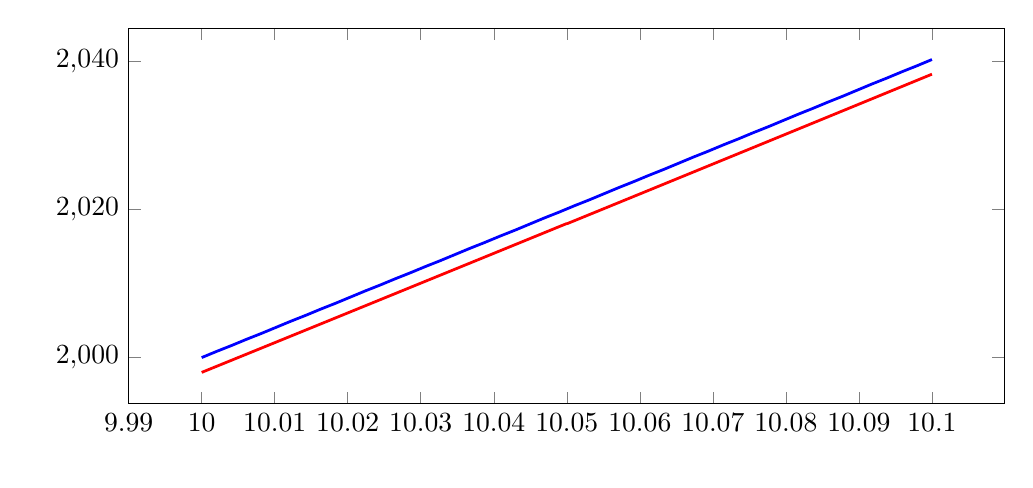
\begin{tikzpicture}[line width=1]
\begin{axis}[width=5in, height=2.5in,
             scatter/classes={a={mark=*,draw=black}},
             xlabel={\mbox{}},
             xlabel style={name=xlabel}, 
             ylabel={\mbox{}}, 
             legend style={
                at={(xlabel.south)},
                yshift=-1ex,
                anchor=north,
                legend cell align=left,
                },
        ]
]
\addplot[draw=red, line width=1] coordinates {(10.0,1998.002)
(10.0001,1998.0421)
(10.0002,1998.0821)
(10.0003,1998.1222)
(10.0004,1998.1622)
(10.0005,1998.2023)
(10.0006,1998.2424)
(10.0007,1998.2824)
(10.0008,1998.3225)
(10.0009,1998.3626)
(10.001,1998.4026)
(10.0011,1998.4427)
(10.0012,1998.4827)
(10.0013,1998.5228)
(10.0014,1998.5629)
(10.0015,1998.6029)
(10.0016,1998.643)
(10.0017,1998.6831)
(10.0018,1998.7231)
(10.0019,1998.7632)
(10.002,1998.8033)
(10.0021,1998.8433)
(10.0022,1998.8834)
(10.0023,1998.9235)
(10.0024,1998.9636)
(10.0025,1999.0036)
(10.0026,1999.0437)
(10.0027,1999.0838)
(10.0028,1999.1238)
(10.0029,1999.1639)
(10.003,1999.204)
(10.0031,1999.244)
(10.0032,1999.2841)
(10.0033,1999.3242)
(10.0034,1999.3643)
(10.0035,1999.4043)
(10.0036,1999.4444)
(10.0037,1999.4845)
(10.0038,1999.5246)
(10.0039,1999.5646)
(10.004,1999.6047)
(10.0041,1999.6448)
(10.0042,1999.6849)
(10.0043,1999.7249)
(10.0044,1999.765)
(10.0045,1999.8051)
(10.0046,1999.8452)
(10.0047,1999.8853)
(10.0048,1999.9253)
(10.0049,1999.9654)
(10.005,2000.0055)
(10.0051,2000.0456)
(10.0052,2000.0857)
(10.0053,2000.1257)
(10.0054,2000.1658)
(10.0055,2000.2059)
(10.0056,2000.246)
(10.0057,2000.2861)
(10.0058,2000.3262)
(10.0059,2000.3662)
(10.006,2000.4063)
(10.0061,2000.4464)
(10.0062,2000.4865)
(10.0063,2000.5266)
(10.0064,2000.5667)
(10.0065,2000.6067)
(10.0066,2000.6468)
(10.0067,2000.6869)
(10.0068,2000.727)
(10.0069,2000.7671)
(10.007,2000.8072)
(10.0071,2000.8473)
(10.0072,2000.8874)
(10.0073,2000.9274)
(10.0074,2000.9675)
(10.0075,2001.0076)
(10.0076,2001.0477)
(10.0077,2001.0878)
(10.0078,2001.1279)
(10.0079,2001.168)
(10.008,2001.2081)
(10.0081,2001.2482)
(10.0082,2001.2883)
(10.0083,2001.3284)
(10.0084,2001.3684)
(10.0085,2001.4085)
(10.0086,2001.4486)
(10.0087,2001.4887)
(10.0088,2001.5288)
(10.0089,2001.5689)
(10.009,2001.609)
(10.0091,2001.6491)
(10.0092,2001.6892)
(10.0093,2001.7293)
(10.0094,2001.7694)
(10.0095,2001.8095)
(10.0096,2001.8496)
(10.0097,2001.8897)
(10.0098,2001.9298)
(10.0099,2001.9699)
(10.01,2002.01)
(10.0101,2002.0501)
(10.0102,2002.0902)
(10.0103,2002.1303)
(10.0104,2002.1704)
(10.0105,2002.2105)
(10.0106,2002.2506)
(10.0107,2002.2907)
(10.0108,2002.3308)
(10.0109,2002.3709)
(10.011,2002.411)
(10.0111,2002.4511)
(10.0112,2002.4912)
(10.0113,2002.5313)
(10.0114,2002.5714)
(10.0115,2002.6115)
(10.0116,2002.6516)
(10.0117,2002.6918)
(10.0118,2002.7319)
(10.0119,2002.772)
(10.012,2002.8121)
(10.0121,2002.8522)
(10.0122,2002.8923)
(10.0123,2002.9324)
(10.0124,2002.9725)
(10.0125,2003.0126)
(10.0126,2003.0527)
(10.0127,2003.0928)
(10.0128,2003.133)
(10.0129,2003.1731)
(10.013,2003.2132)
(10.0131,2003.2533)
(10.0132,2003.2934)
(10.0133,2003.3335)
(10.0134,2003.3736)
(10.0135,2003.4137)
(10.0136,2003.4539)
(10.0137,2003.494)
(10.0138,2003.5341)
(10.0139,2003.5742)
(10.014,2003.6143)
(10.0141,2003.6544)
(10.0142,2003.6946)
(10.0143,2003.7347)
(10.0144,2003.7748)
(10.0145,2003.8149)
(10.0146,2003.855)
(10.0147,2003.8951)
(10.0148,2003.9353)
(10.0149,2003.9754)
(10.015,2004.0155)
(10.0151,2004.0556)
(10.0152,2004.0957)
(10.0153,2004.1359)
(10.0154,2004.176)
(10.0155,2004.2161)
(10.0156,2004.2562)
(10.0157,2004.2963)
(10.0158,2004.3365)
(10.0159,2004.3766)
(10.016,2004.4167)
(10.0161,2004.4568)
(10.0162,2004.497)
(10.0163,2004.5371)
(10.0164,2004.5772)
(10.0165,2004.6173)
(10.0166,2004.6575)
(10.0167,2004.6976)
(10.0168,2004.7377)
(10.0169,2004.7779)
(10.017,2004.818)
(10.0171,2004.8581)
(10.0172,2004.8982)
(10.0173,2004.9384)
(10.0174,2004.9785)
(10.0175,2005.0186)
(10.0176,2005.0588)
(10.0177,2005.0989)
(10.0178,2005.139)
(10.0179,2005.1791)
(10.018,2005.2193)
(10.0181,2005.2594)
(10.0182,2005.2995)
(10.0183,2005.3397)
(10.0184,2005.3798)
(10.0185,2005.4199)
(10.0186,2005.4601)
(10.0187,2005.5002)
(10.0188,2005.5404)
(10.0189,2005.5805)
(10.019,2005.6206)
(10.0191,2005.6608)
(10.0192,2005.7009)
(10.0193,2005.741)
(10.0194,2005.7812)
(10.0195,2005.8213)
(10.0196,2005.8614)
(10.0197,2005.9016)
(10.0198,2005.9417)
(10.0199,2005.9819)
(10.02,2006.022)
(10.0201,2006.0621)
(10.0202,2006.1023)
(10.0203,2006.1424)
(10.0204,2006.1826)
(10.0205,2006.2227)
(10.0206,2006.2628)
(10.0207,2006.303)
(10.0208,2006.3431)
(10.0209,2006.3833)
(10.021,2006.4234)
(10.0211,2006.4636)
(10.0212,2006.5037)
(10.0213,2006.5439)
(10.0214,2006.584)
(10.0215,2006.6241)
(10.0216,2006.6643)
(10.0217,2006.7044)
(10.0218,2006.7446)
(10.0219,2006.7847)
(10.022,2006.8249)
(10.0221,2006.865)
(10.0222,2006.9052)
(10.0223,2006.9453)
(10.0224,2006.9855)
(10.0225,2007.0256)
(10.0226,2007.0658)
(10.0227,2007.1059)
(10.0228,2007.1461)
(10.0229,2007.1862)
(10.023,2007.2264)
(10.0231,2007.2665)
(10.0232,2007.3067)
(10.0233,2007.3468)
(10.0234,2007.387)
(10.0235,2007.4271)
(10.0236,2007.4673)
(10.0237,2007.5075)
(10.0238,2007.5476)
(10.0239,2007.5878)
(10.024,2007.6279)
(10.0241,2007.6681)
(10.0242,2007.7082)
(10.0243,2007.7484)
(10.0244,2007.7886)
(10.0245,2007.8287)
(10.0246,2007.8689)
(10.0247,2007.909)
(10.0248,2007.9492)
(10.0249,2007.9893)
(10.025,2008.0295)
(10.0251,2008.0697)
(10.0252,2008.1098)
(10.0253,2008.15)
(10.0254,2008.1901)
(10.0255,2008.2303)
(10.0256,2008.2705)
(10.0257,2008.3106)
(10.0258,2008.3508)
(10.0259,2008.391)
(10.026,2008.4311)
(10.0261,2008.4713)
(10.0262,2008.5115)
(10.0263,2008.5516)
(10.0264,2008.5918)
(10.0265,2008.632)
(10.0266,2008.6721)
(10.0267,2008.7123)
(10.0268,2008.7525)
(10.0269,2008.7926)
(10.027,2008.8328)
(10.0271,2008.873)
(10.0272,2008.9131)
(10.0273,2008.9533)
(10.0274,2008.9935)
(10.0275,2009.0336)
(10.0276,2009.0738)
(10.0277,2009.114)
(10.0278,2009.1541)
(10.0279,2009.1943)
(10.028,2009.2345)
(10.0281,2009.2747)
(10.0282,2009.3148)
(10.0283,2009.355)
(10.0284,2009.3952)
(10.0285,2009.4354)
(10.0286,2009.4755)
(10.0287,2009.5157)
(10.0288,2009.5559)
(10.0289,2009.5961)
(10.029,2009.6362)
(10.0291,2009.6764)
(10.0292,2009.7166)
(10.0293,2009.7568)
(10.0294,2009.7969)
(10.0295,2009.8371)
(10.0296,2009.8773)
(10.0297,2009.9175)
(10.0298,2009.9577)
(10.0299,2009.9978)
(10.03,2010.038)
(10.0301,2010.0782)
(10.0302,2010.1184)
(10.0303,2010.1586)
(10.0304,2010.1987)
(10.0305,2010.2389)
(10.0306,2010.2791)
(10.0307,2010.3193)
(10.0308,2010.3595)
(10.0309,2010.3996)
(10.031,2010.4398)
(10.0311,2010.48)
(10.0312,2010.5202)
(10.0313,2010.5604)
(10.0314,2010.6006)
(10.0315,2010.6408)
(10.0316,2010.6809)
(10.0317,2010.7211)
(10.0318,2010.7613)
(10.0319,2010.8015)
(10.032,2010.8417)
(10.0321,2010.8819)
(10.0322,2010.9221)
(10.0323,2010.9623)
(10.0324,2011.0024)
(10.0325,2011.0426)
(10.0326,2011.0828)
(10.0327,2011.123)
(10.0328,2011.1632)
(10.0329,2011.2034)
(10.033,2011.2436)
(10.0331,2011.2838)
(10.0332,2011.324)
(10.0333,2011.3642)
(10.0334,2011.4044)
(10.0335,2011.4446)
(10.0336,2011.4848)
(10.0337,2011.5249)
(10.0338,2011.5651)
(10.0339,2011.6053)
(10.034,2011.6455)
(10.0341,2011.6857)
(10.0342,2011.7259)
(10.0343,2011.7661)
(10.0344,2011.8063)
(10.0345,2011.8465)
(10.0346,2011.8867)
(10.0347,2011.9269)
(10.0348,2011.9671)
(10.0349,2012.0073)
(10.035,2012.0475)
(10.0351,2012.0877)
(10.0352,2012.1279)
(10.0353,2012.1681)
(10.0354,2012.2083)
(10.0355,2012.2485)
(10.0356,2012.2887)
(10.0357,2012.3289)
(10.0358,2012.3691)
(10.0359,2012.4093)
(10.036,2012.4495)
(10.0361,2012.4897)
(10.0362,2012.5299)
(10.0363,2012.5702)
(10.0364,2012.6104)
(10.0365,2012.6506)
(10.0366,2012.6908)
(10.0367,2012.731)
(10.0368,2012.7712)
(10.0369,2012.8114)
(10.037,2012.8516)
(10.0371,2012.8918)
(10.0372,2012.932)
(10.0373,2012.9722)
(10.0374,2013.0124)
(10.0375,2013.0526)
(10.0376,2013.0929)
(10.0377,2013.1331)
(10.0378,2013.1733)
(10.0379,2013.2135)
(10.038,2013.2537)
(10.0381,2013.2939)
(10.0382,2013.3341)
(10.0383,2013.3743)
(10.0384,2013.4146)
(10.0385,2013.4548)
(10.0386,2013.495)
(10.0387,2013.5352)
(10.0388,2013.5754)
(10.0389,2013.6156)
(10.039,2013.6558)
(10.0391,2013.6961)
(10.0392,2013.7363)
(10.0393,2013.7765)
(10.0394,2013.8167)
(10.0395,2013.8569)
(10.0396,2013.8971)
(10.0397,2013.9374)
(10.0398,2013.9776)
(10.0399,2014.0178)
(10.04,2014.058)
(10.0401,2014.0982)
(10.0402,2014.1385)
(10.0403,2014.1787)
(10.0404,2014.2189)
(10.0405,2014.2591)
(10.0406,2014.2994)
(10.0407,2014.3396)
(10.0408,2014.3798)
(10.0409,2014.42)
(10.041,2014.4602)
(10.0411,2014.5005)
(10.0412,2014.5407)
(10.0413,2014.5809)
(10.0414,2014.6211)
(10.0415,2014.6614)
(10.0416,2014.7016)
(10.0417,2014.7418)
(10.0418,2014.782)
(10.0419,2014.8223)
(10.042,2014.8625)
(10.0421,2014.9027)
(10.0422,2014.943)
(10.0423,2014.9832)
(10.0424,2015.0234)
(10.0425,2015.0637)
(10.0426,2015.1039)
(10.0427,2015.1441)
(10.0428,2015.1843)
(10.0429,2015.2246)
(10.043,2015.2648)
(10.0431,2015.305)
(10.0432,2015.3453)
(10.0433,2015.3855)
(10.0434,2015.4257)
(10.0435,2015.466)
(10.0436,2015.5062)
(10.0437,2015.5464)
(10.0438,2015.5867)
(10.0439,2015.6269)
(10.044,2015.6671)
(10.0441,2015.7074)
(10.0442,2015.7476)
(10.0443,2015.7879)
(10.0444,2015.8281)
(10.0445,2015.8683)
(10.0446,2015.9086)
(10.0447,2015.9488)
(10.0448,2015.9891)
(10.0449,2016.0293)
(10.045,2016.0695)
(10.0451,2016.1098)
(10.0452,2016.15)
(10.0453,2016.1903)
(10.0454,2016.2305)
(10.0455,2016.2707)
(10.0456,2016.311)
(10.0457,2016.3512)
(10.0458,2016.3915)
(10.0459,2016.4317)
(10.046,2016.472)
(10.0461,2016.5122)
(10.0462,2016.5524)
(10.0463,2016.5927)
(10.0464,2016.6329)
(10.0465,2016.6732)
(10.0466,2016.7134)
(10.0467,2016.7537)
(10.0468,2016.7939)
(10.0469,2016.8342)
(10.047,2016.8744)
(10.0471,2016.9147)
(10.0472,2016.9549)
(10.0473,2016.9952)
(10.0474,2017.0354)
(10.0475,2017.0757)
(10.0476,2017.1159)
(10.0477,2017.1562)
(10.0478,2017.1964)
(10.0479,2017.2367)
(10.048,2017.2769)
(10.0481,2017.3172)
(10.0482,2017.3574)
(10.0483,2017.3977)
(10.0484,2017.4379)
(10.0485,2017.4782)
(10.0486,2017.5184)
(10.0487,2017.5587)
(10.0488,2017.5989)
(10.0489,2017.6392)
(10.049,2017.6795)
(10.0491,2017.7197)
(10.0492,2017.76)
(10.0493,2017.8002)
(10.0494,2017.8405)
(10.0495,2017.8807)
(10.0496,2017.921)
(10.0497,2017.9613)
(10.0498,2018.0015)
(10.0499,2018.0418)
(10.0501,2018.082)
(10.0502,2018.1223)
(10.0503,2018.1626)
(10.0504,2018.2028)
(10.0505,2018.2431)
(10.0506,2018.2833)
(10.0507,2018.3236)
(10.0508,2018.3639)
(10.0509,2018.4041)
(10.051,2018.4444)
(10.0511,2018.4847)
(10.0512,2018.5249)
(10.0513,2018.5652)
(10.0514,2018.6055)
(10.0515,2018.6457)
(10.0516,2018.686)
(10.0517,2018.7263)
(10.0518,2018.7665)
(10.0519,2018.8068)
(10.052,2018.8471)
(10.0521,2018.8873)
(10.0522,2018.9276)
(10.0523,2018.9679)
(10.0524,2019.0081)
(10.0525,2019.0484)
(10.0526,2019.0887)
(10.0527,2019.1289)
(10.0528,2019.1692)
(10.0529,2019.2095)
(10.053,2019.2498)
(10.0531,2019.29)
(10.0532,2019.3303)
(10.0533,2019.3706)
(10.0534,2019.4108)
(10.0535,2019.4511)
(10.0536,2019.4914)
(10.0537,2019.5317)
(10.0538,2019.5719)
(10.0539,2019.6122)
(10.054,2019.6525)
(10.0541,2019.6928)
(10.0542,2019.733)
(10.0543,2019.7733)
(10.0544,2019.8136)
(10.0545,2019.8539)
(10.0546,2019.8942)
(10.0547,2019.9344)
(10.0548,2019.9747)
(10.0549,2020.015)
(10.055,2020.0553)
(10.0551,2020.0955)
(10.0552,2020.1358)
(10.0553,2020.1761)
(10.0554,2020.2164)
(10.0555,2020.2567)
(10.0556,2020.297)
(10.0557,2020.3372)
(10.0558,2020.3775)
(10.0559,2020.4178)
(10.056,2020.4581)
(10.0561,2020.4984)
(10.0562,2020.5387)
(10.0563,2020.5789)
(10.0564,2020.6192)
(10.0565,2020.6595)
(10.0566,2020.6998)
(10.0567,2020.7401)
(10.0568,2020.7804)
(10.0569,2020.8207)
(10.057,2020.8609)
(10.0571,2020.9012)
(10.0572,2020.9415)
(10.0573,2020.9818)
(10.0574,2021.0221)
(10.0575,2021.0624)
(10.0576,2021.1027)
(10.0577,2021.143)
(10.0578,2021.1833)
(10.0579,2021.2236)
(10.058,2021.2638)
(10.0581,2021.3041)
(10.0582,2021.3444)
(10.0583,2021.3847)
(10.0584,2021.425)
(10.0585,2021.4653)
(10.0586,2021.5056)
(10.0587,2021.5459)
(10.0588,2021.5862)
(10.0589,2021.6265)
(10.059,2021.6668)
(10.0591,2021.7071)
(10.0592,2021.7474)
(10.0593,2021.7877)
(10.0594,2021.828)
(10.0595,2021.8683)
(10.0596,2021.9086)
(10.0597,2021.9489)
(10.0598,2021.9892)
(10.0599,2022.0295)
(10.06,2022.0698)
(10.0601,2022.1101)
(10.0602,2022.1504)
(10.0603,2022.1907)
(10.0604,2022.231)
(10.0605,2022.2713)
(10.0606,2022.3116)
(10.0607,2022.3519)
(10.0608,2022.3922)
(10.0609,2022.4325)
(10.061,2022.4728)
(10.0611,2022.5131)
(10.0612,2022.5534)
(10.0613,2022.5937)
(10.0614,2022.634)
(10.0615,2022.6743)
(10.0616,2022.7146)
(10.0617,2022.7549)
(10.0618,2022.7952)
(10.0619,2022.8355)
(10.062,2022.8758)
(10.0621,2022.9161)
(10.0622,2022.9565)
(10.0623,2022.9968)
(10.0624,2023.0371)
(10.0625,2023.0774)
(10.0626,2023.1177)
(10.0627,2023.158)
(10.0628,2023.1983)
(10.0629,2023.2386)
(10.063,2023.2789)
(10.0631,2023.3192)
(10.0632,2023.3596)
(10.0633,2023.3999)
(10.0634,2023.4402)
(10.0635,2023.4805)
(10.0636,2023.5208)
(10.0637,2023.5611)
(10.0638,2023.6014)
(10.0639,2023.6418)
(10.064,2023.6821)
(10.0641,2023.7224)
(10.0642,2023.7627)
(10.0643,2023.803)
(10.0644,2023.8433)
(10.0645,2023.8837)
(10.0646,2023.924)
(10.0647,2023.9643)
(10.0648,2024.0046)
(10.0649,2024.0449)
(10.065,2024.0853)
(10.0651,2024.1256)
(10.0652,2024.1659)
(10.0653,2024.2062)
(10.0654,2024.2465)
(10.0655,2024.2869)
(10.0656,2024.3272)
(10.0657,2024.3675)
(10.0658,2024.4078)
(10.0659,2024.4481)
(10.066,2024.4885)
(10.0661,2024.5288)
(10.0662,2024.5691)
(10.0663,2024.6094)
(10.0664,2024.6498)
(10.0665,2024.6901)
(10.0666,2024.7304)
(10.0667,2024.7707)
(10.0668,2024.8111)
(10.0669,2024.8514)
(10.067,2024.8917)
(10.0671,2024.9321)
(10.0672,2024.9724)
(10.0673,2025.0127)
(10.0674,2025.053)
(10.0675,2025.0934)
(10.0676,2025.1337)
(10.0677,2025.174)
(10.0678,2025.2144)
(10.0679,2025.2547)
(10.068,2025.295)
(10.0681,2025.3354)
(10.0682,2025.3757)
(10.0683,2025.416)
(10.0684,2025.4564)
(10.0685,2025.4967)
(10.0686,2025.537)
(10.0687,2025.5774)
(10.0688,2025.6177)
(10.0689,2025.658)
(10.069,2025.6984)
(10.0691,2025.7387)
(10.0692,2025.779)
(10.0693,2025.8194)
(10.0694,2025.8597)
(10.0695,2025.9)
(10.0696,2025.9404)
(10.0697,2025.9807)
(10.0698,2026.0211)
(10.0699,2026.0614)
(10.07,2026.1017)
(10.0701,2026.1421)
(10.0702,2026.1824)
(10.0703,2026.2228)
(10.0704,2026.2631)
(10.0705,2026.3034)
(10.0706,2026.3438)
(10.0707,2026.3841)
(10.0708,2026.4245)
(10.0709,2026.4648)
(10.071,2026.5052)
(10.0711,2026.5455)
(10.0712,2026.5859)
(10.0713,2026.6262)
(10.0714,2026.6665)
(10.0715,2026.7069)
(10.0716,2026.7472)
(10.0717,2026.7876)
(10.0718,2026.8279)
(10.0719,2026.8683)
(10.072,2026.9086)
(10.0721,2026.949)
(10.0722,2026.9893)
(10.0723,2027.0297)
(10.0724,2027.07)
(10.0725,2027.1104)
(10.0726,2027.1507)
(10.0727,2027.1911)
(10.0728,2027.2314)
(10.0729,2027.2718)
(10.073,2027.3121)
(10.0731,2027.3525)
(10.0732,2027.3928)
(10.0733,2027.4332)
(10.0734,2027.4735)
(10.0735,2027.5139)
(10.0736,2027.5542)
(10.0737,2027.5946)
(10.0738,2027.6349)
(10.0739,2027.6753)
(10.074,2027.7157)
(10.0741,2027.756)
(10.0742,2027.7964)
(10.0743,2027.8367)
(10.0744,2027.8771)
(10.0745,2027.9174)
(10.0746,2027.9578)
(10.0747,2027.9982)
(10.0748,2028.0385)
(10.0749,2028.0789)
(10.075,2028.1192)
(10.0751,2028.1596)
(10.0752,2028.2)
(10.0753,2028.2403)
(10.0754,2028.2807)
(10.0755,2028.321)
(10.0756,2028.3614)
(10.0757,2028.4018)
(10.0758,2028.4421)
(10.0759,2028.4825)
(10.076,2028.5229)
(10.0761,2028.5632)
(10.0762,2028.6036)
(10.0763,2028.6439)
(10.0764,2028.6843)
(10.0765,2028.7247)
(10.0766,2028.765)
(10.0767,2028.8054)
(10.0768,2028.8458)
(10.0769,2028.8861)
(10.077,2028.9265)
(10.0771,2028.9669)
(10.0772,2029.0073)
(10.0773,2029.0476)
(10.0774,2029.088)
(10.0775,2029.1284)
(10.0776,2029.1687)
(10.0777,2029.2091)
(10.0778,2029.2495)
(10.0779,2029.2898)
(10.078,2029.3302)
(10.0781,2029.3706)
(10.0782,2029.411)
(10.0783,2029.4513)
(10.0784,2029.4917)
(10.0785,2029.5321)
(10.0786,2029.5725)
(10.0787,2029.6128)
(10.0788,2029.6532)
(10.0789,2029.6936)
(10.079,2029.734)
(10.0791,2029.7743)
(10.0792,2029.8147)
(10.0793,2029.8551)
(10.0794,2029.8955)
(10.0795,2029.9358)
(10.0796,2029.9762)
(10.0797,2030.0166)
(10.0798,2030.057)
(10.0799,2030.0974)
(10.08,2030.1377)
(10.0801,2030.1781)
(10.0802,2030.2185)
(10.0803,2030.2589)
(10.0804,2030.2993)
(10.0805,2030.3396)
(10.0806,2030.38)
(10.0807,2030.4204)
(10.0808,2030.4608)
(10.0809,2030.5012)
(10.081,2030.5416)
(10.0811,2030.5819)
(10.0812,2030.6223)
(10.0813,2030.6627)
(10.0814,2030.7031)
(10.0815,2030.7435)
(10.0816,2030.7839)
(10.0817,2030.8242)
(10.0818,2030.8646)
(10.0819,2030.905)
(10.082,2030.9454)
(10.0821,2030.9858)
(10.0822,2031.0262)
(10.0823,2031.0666)
(10.0824,2031.107)
(10.0825,2031.1474)
(10.0826,2031.1877)
(10.0827,2031.2281)
(10.0828,2031.2685)
(10.0829,2031.3089)
(10.083,2031.3493)
(10.0831,2031.3897)
(10.0832,2031.4301)
(10.0833,2031.4705)
(10.0834,2031.5109)
(10.0835,2031.5513)
(10.0836,2031.5917)
(10.0837,2031.6321)
(10.0838,2031.6725)
(10.0839,2031.7129)
(10.084,2031.7532)
(10.0841,2031.7936)
(10.0842,2031.834)
(10.0843,2031.8744)
(10.0844,2031.9148)
(10.0845,2031.9552)
(10.0846,2031.9956)
(10.0847,2032.036)
(10.0848,2032.0764)
(10.0849,2032.1168)
(10.085,2032.1572)
(10.0851,2032.1976)
(10.0852,2032.238)
(10.0853,2032.2784)
(10.0854,2032.3188)
(10.0855,2032.3592)
(10.0856,2032.3996)
(10.0857,2032.44)
(10.0858,2032.4804)
(10.0859,2032.5208)
(10.086,2032.5612)
(10.0861,2032.6017)
(10.0862,2032.6421)
(10.0863,2032.6825)
(10.0864,2032.7229)
(10.0865,2032.7633)
(10.0866,2032.8037)
(10.0867,2032.8441)
(10.0868,2032.8845)
(10.0869,2032.9249)
(10.087,2032.9653)
(10.0871,2033.0057)
(10.0872,2033.0461)
(10.0873,2033.0865)
(10.0874,2033.1269)
(10.0875,2033.1674)
(10.0876,2033.2078)
(10.0877,2033.2482)
(10.0878,2033.2886)
(10.0879,2033.329)
(10.088,2033.3694)
(10.0881,2033.4098)
(10.0882,2033.4502)
(10.0883,2033.4906)
(10.0884,2033.5311)
(10.0885,2033.5715)
(10.0886,2033.6119)
(10.0887,2033.6523)
(10.0888,2033.6927)
(10.0889,2033.7331)
(10.089,2033.7735)
(10.0891,2033.814)
(10.0892,2033.8544)
(10.0893,2033.8948)
(10.0894,2033.9352)
(10.0895,2033.9756)
(10.0896,2034.016)
(10.0897,2034.0565)
(10.0898,2034.0969)
(10.0899,2034.1373)
(10.09,2034.1777)
(10.0901,2034.2181)
(10.0902,2034.2586)
(10.0903,2034.299)
(10.0904,2034.3394)
(10.0905,2034.3798)
(10.0906,2034.4203)
(10.0907,2034.4607)
(10.0908,2034.5011)
(10.0909,2034.5415)
(10.091,2034.5819)
(10.0911,2034.6224)
(10.0912,2034.6628)
(10.0913,2034.7032)
(10.0914,2034.7436)
(10.0915,2034.7841)
(10.0916,2034.8245)
(10.0917,2034.8649)
(10.0918,2034.9053)
(10.0919,2034.9458)
(10.092,2034.9862)
(10.0921,2035.0266)
(10.0922,2035.0671)
(10.0923,2035.1075)
(10.0924,2035.1479)
(10.0925,2035.1883)
(10.0926,2035.2288)
(10.0927,2035.2692)
(10.0928,2035.3096)
(10.0929,2035.3501)
(10.093,2035.3905)
(10.0931,2035.4309)
(10.0932,2035.4714)
(10.0933,2035.5118)
(10.0934,2035.5522)
(10.0935,2035.5927)
(10.0936,2035.6331)
(10.0937,2035.6735)
(10.0938,2035.714)
(10.0939,2035.7544)
(10.094,2035.7948)
(10.0941,2035.8353)
(10.0942,2035.8757)
(10.0943,2035.9162)
(10.0944,2035.9566)
(10.0945,2035.997)
(10.0946,2036.0375)
(10.0947,2036.0779)
(10.0948,2036.1183)
(10.0949,2036.1588)
(10.095,2036.1992)
(10.0951,2036.2397)
(10.0952,2036.2801)
(10.0953,2036.3205)
(10.0954,2036.361)
(10.0955,2036.4014)
(10.0956,2036.4419)
(10.0957,2036.4823)
(10.0958,2036.5228)
(10.0959,2036.5632)
(10.096,2036.6036)
(10.0961,2036.6441)
(10.0962,2036.6845)
(10.0963,2036.725)
(10.0964,2036.7654)
(10.0965,2036.8059)
(10.0966,2036.8463)
(10.0967,2036.8868)
(10.0968,2036.9272)
(10.0969,2036.9677)
(10.097,2037.0081)
(10.0971,2037.0486)
(10.0972,2037.089)
(10.0973,2037.1294)
(10.0974,2037.1699)
(10.0975,2037.2103)
(10.0976,2037.2508)
(10.0977,2037.2912)
(10.0978,2037.3317)
(10.0979,2037.3722)
(10.098,2037.4126)
(10.0981,2037.4531)
(10.0982,2037.4935)
(10.0983,2037.534)
(10.0984,2037.5744)
(10.0985,2037.6149)
(10.0986,2037.6553)
(10.0987,2037.6958)
(10.0988,2037.7362)
(10.0989,2037.7767)
(10.099,2037.8171)
(10.0991,2037.8576)
(10.0992,2037.8981)
(10.0993,2037.9385)
(10.0994,2037.979)
(10.0995,2038.0194)
(10.0996,2038.0599)
(10.0997,2038.1003)
(10.0998,2038.1408)
(10.0999,2038.1813)
(10.1,2038.2217)};\node[pin=below right:{$y=|20 \frac{n^5}{n^3 + 1}|$}] at (axis cs:10.5,2203.0968820800517) {};\addplot[draw=blue, line width=1] coordinates {(10.0,2000.0)
(10.002,2000.8164)
(10.0041,2001.633)
(10.0061,2002.4497)
(10.0082,2003.2666)
(10.0102,2004.0837)
(10.0122,2004.901)
(10.0143,2005.7184)
(10.0163,2006.5359)
(10.0184,2007.3537)
(10.0204,2008.1716)
(10.0224,2008.9897)
(10.0245,2009.8079)
(10.0265,2010.6263)
(10.0286,2011.4449)
(10.0306,2012.2636)
(10.0327,2013.0825)
(10.0347,2013.9016)
(10.0367,2014.7209)
(10.0388,2015.5403)
(10.0408,2016.3599)
(10.0429,2017.1796)
(10.0449,2017.9995)
(10.0469,2018.8196)
(10.049,2019.6398)
(10.051,2020.4602)
(10.0531,2021.2808)
(10.0551,2022.1015)
(10.0571,2022.9224)
(10.0592,2023.7435)
(10.0612,2024.5648)
(10.0633,2025.3862)
(10.0653,2026.2077)
(10.0673,2027.0295)
(10.0694,2027.8514)
(10.0714,2028.6735)
(10.0735,2029.4957)
(10.0755,2030.3181)
(10.0776,2031.1407)
(10.0796,2031.9634)
(10.0816,2032.7863)
(10.0837,2033.6094)
(10.0857,2034.4327)
(10.0878,2035.2561)
(10.0898,2036.0796)
(10.0918,2036.9034)
(10.0939,2037.7273)
(10.0959,2038.5514)
(10.098,2039.3756)
(10.1,2040.2)};\node[pin=above left:{$y=20n^2$}] at (axis cs:10.5,2205.0) {};
\end{axis}\end{tikzpicture}\end{center}

he blue graph of $20n^2$ is above the red graph of $f(n)$
on the interval $[10, 10.1]$.
By zooming in at different places on the positive part of the real
axis, we see that the blue graph is always above the red graph.
In fact
\[
|f_0(n)| \leq 20n^2
\]
for all $n > 0$.
This can be proven mathematically:
If $n > 0$, then
\[
n^3 < n^3 + 1
\]
Therefore
\[
\frac{1}{n^3 + 1} < \frac{1}{n^3}
\]
and hence
\[
20 \frac{n^5}{n^3 + 1} < 20 \frac{n^5}{n^3} = 20 n^2
\]
Therefore if we choose $C_0 = 20$ and $N_0 = 1$,
we see that for $n \geq N_0$,
\[
\left|
20 \frac{n^5}{n^3 + 1}
\right| 
\leq C_0
\left|
n^2
\right|
\]
i.e.,
\[
|f_0(n)| \leq C_0|g(n)|
\]
Hence
\[
f_0(n) = O(n^2)
\]

(b)
Let $f_1(n) = 5n^3\cos(n)$.
The following are plots of $|f_1(n)|$ (in red) and $5n^3$:
%-*-latex-*-

\begin{center}
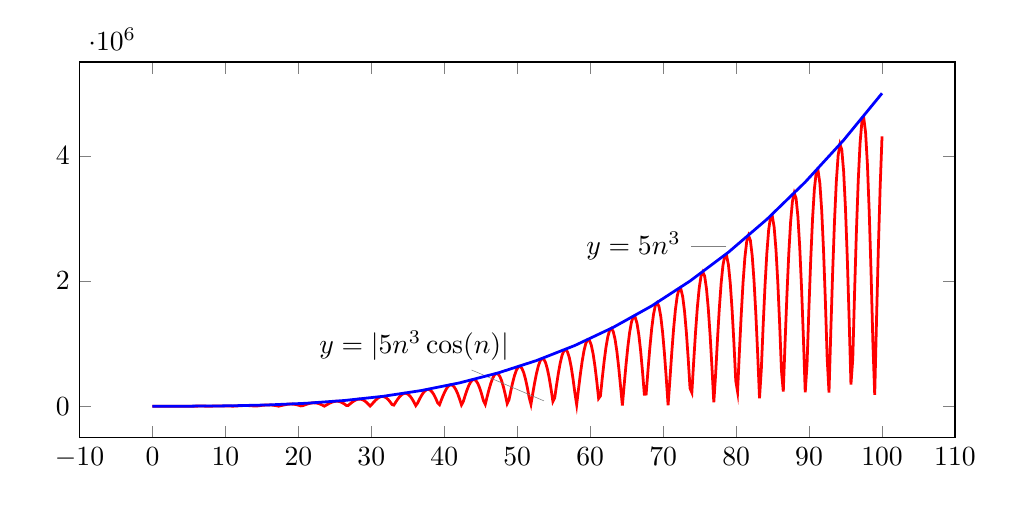
\begin{tikzpicture}[line width=1]
\begin{axis}[width=5in, height=2.5in,
             scatter/classes={a={mark=*,draw=black}},
             xlabel={\mbox{}},
             xlabel style={name=xlabel}, 
             ylabel={\mbox{}}, 
             legend style={
                at={(xlabel.south)},
                yshift=-1ex,
                anchor=north,
                legend cell align=left,
                },
        ]
]
\addplot[draw=red, line width=1] coordinates {(0.0,0.0)
(0.2506,0.0763)
(0.5013,0.5522)
(0.7519,1.5523)
(1.0025,2.7112)
(1.2531,3.0733)
(1.5038,1.1389)
(1.7544,4.9289)
(2.005,16.9548)
(2.2556,36.2973)
(2.5063,63.355)
(2.7569,97.1108)
(3.0075,134.7969)
(3.2581,171.7611)
(3.5088,201.5937)
(3.7594,216.5526)
(4.01,208.2859)
(4.2607,168.8152)
(4.5113,91.7007)
(4.7619,26.7226)
(5.0125,186.178)
(5.2632,381.5007)
(5.5138,602.063)
(5.7644,831.7033)
(6.015,1049.2541)
(6.2657,1229.7156)
(6.5163,1346.0573)
(6.7669,1371.5641)
(7.0175,1282.5724)
(7.2682,1061.3843)
(7.5188,699.0954)
(7.7694,198.0495)
(8.0201,426.3737)
(8.2707,1144.906)
(8.5213,1914.6862)
(8.7719,2680.8415)
(9.0226,3379.3878)
(9.2732,3941.368)
(9.5238,4298.0256)
(9.7744,4386.6931)
(10.0251,4156.9736)
(10.2757,3576.719)
(10.5263,2637.2653)
(10.7769,1357.3907)
(11.0276,214.4926)
(11.2782,2000.3067)
(11.5288,3894.691)
(11.7794,5769.8841)
(12.0301,7482.9906)
(12.2807,8885.308)
(12.5313,9833.1944)
(12.782,10199.7711)
(13.0326,9886.6226)
(13.2832,8834.5691)
(13.5338,7032.569)
(13.7845,4523.8674)
(14.0351,1408.6343)
(14.2857,2157.4582)
(14.5363,5969.008)
(14.787,9780.9831)
(15.0376,13322.7913)
(15.2882,16315.6277)
(15.5388,18492.0937)
(15.7895,19616.822)
(16.0401,19506.6556)
(16.2907,18048.8376)
(16.5414,15215.6878)
(16.792,11074.3758)
(17.0426,5790.6524)
(17.2932,374.2455)
(17.5439,7073.8589)
(17.7945,13893.7811)
(18.0451,20375.2581)
(18.2957,26043.91)
(18.5464,30441.9077)
(18.797,33161.5538)
(19.0476,33877.9669)
(19.2982,32378.4552)
(19.5489,28586.2311)
(19.7995,22576.3511)
(20.0501,14582.1731)
(20.3008,4991.1776)
(20.5514,5670.3211)
(20.802,16763.2878)
(21.0526,27571.8321)
(21.3033,37346.9858)
(21.5539,45355.8698)
(21.8045,50933.1757)
(22.0551,53531.5218)
(22.3058,52767.095)
(22.5564,48457.0873)
(22.807,40645.785)
(23.0576,29616.7626)
(23.3083,15889.4411)
(23.5589,199.251)
(23.8095,16538.266)
(24.0602,33277.9478)
(24.3108,48907.524)
(24.5614,62318.5914)
(24.812,72481.6988)
(25.0627,78520.6432)
(25.3133,79780.8477)
(25.5639,75886.801)
(25.8145,66783.9973)
(26.0652,52761.6217)
(26.3158,34453.3308)
(26.5664,12814.8258)
(26.817,10921.5658)
(27.0677,35313.5094)
(27.3183,58793.1453)
(27.5689,79764.7012)
(27.8195,96709.3532)
(28.0702,108290.6501)
(28.3208,113453.421)
(28.5714,111509.1585)
(28.8221,102201.4189)
(29.0727,85745.8)
(29.3233,62840.4934)
(29.5739,34645.1939)
(29.8246,2728.1651)
(30.0752,31016.6014)
(30.3258,64478.0898)
(30.5764,95456.8453)
(30.8271,121805.8331)
(31.0777,141574.7699)
(31.3283,153148.4713)
(31.5789,155369.7079)
(31.8296,147637.6489)
(32.0802,129974.1848)
(32.3308,103052.2069)
(32.5815,68182.1851)
(32.8321,27256.0026)
(33.0827,17350.1992)
(33.3333,62909.5949)
(33.584,106507.4766)
(33.8346,145223.8187)
(34.0852,176324.4133)
(34.3358,197448.3196)
(34.5865,206779.0794)
(34.8371,203187.6808)
(35.0877,186336.6092)
(35.3383,156736.441)
(35.589,115749.2164)
(35.8396,65536.1026)
(36.0902,8950.4362)
(36.3409,50619.1093)
(36.5915,109446.9991)
(36.8421,163699.6336)
(37.0927,209680.6848)
(37.3434,244077.5372)
(37.594,264192.7061)
(37.8446,268144.4457)
(38.0952,255022.1602)
(38.3459,224984.6319)
(38.5965,179292.3703)
(38.8471,120269.3725)
(39.0977,51194.0407)
(39.3484,23876.3609)
(39.599,100338.794)
(39.8496,173322.0555)
(40.1003,237992.4668)
(40.3509,289868.748)
(40.6015,325125.8696)
(40.8521,340867.646)
(41.1028,335349.1288)
(41.3534,308132.449)
(41.604,260163.5052)
(41.8546,193761.6128)
(42.1053,112519.6283)
(42.3559,21117.8178)
(42.6065,74939.5124)
(42.8571,169650.2485)
(43.1078,256884.582)
(43.3584,330776.4936)
(43.609,386111.9194)
(43.8596,418688.2714)
(44.1103,425620.9749)
(44.3609,405575.2984)
(44.6115,358905.8734)
(44.8622,287691.7059)
(45.1128,195660.8683)
(45.3634,88006.0344)
(45.614,28900.8461)
(45.8647,147879.6108)
(46.1153,261377.4951)
(46.3659,361943.2114)
(46.6165,442710.0727)
(46.8672,497857.1899)
(47.1178,523018.1948)
(47.3684,515609.3588)
(47.619,475053.3051)
(47.8697,402880.5146)
(48.1203,302698.1859)
(48.3709,180024.2655)
(48.6216,41993.1279)
(48.8722,103052.1033)
(49.1228,246057.8051)
(49.3734,377819.3212)
(49.6241,489567.4324)
(49.8747,573544.8237)
(50.1253,623535.0658)
(50.3759,635308.5597)
(50.6266,606954.1891)
(50.8772,539071.8708)
(51.1278,434809.4348)
(51.3784,299736.827)
(51.6291,141560.917)
(51.8797,30305.4222)
(52.1303,205296.4948)
(52.381,372337.187)
(52.6316,520537.8134)
(52.8822,639897.1873)
(53.1328,721968.9271)
(53.3835,760447.095)
(53.6341,751631.2117)
(53.8847,694737.3315)
(54.1353,592030.8359)
(54.386,448767.4013)
(54.6366,272940.5637)
(54.8872,74846.7108)
(55.1378,133509.6229)
(55.3885,339136.3801)
(55.6391,528857.7163)
(55.8897,690151.5318)
(56.1404,811967.9669)
(56.391,885475.8259)
(56.6416,904687.0969)
(56.8922,866916.2323)
(57.1429,773040.3147)
(57.3935,627538.1223)
(57.6441,438299.7268)
(57.8947,216212.7688)
(58.1454,25453.9409)
(58.396,271835.3033)
(58.6466,507377.3956)
(58.8972,716812.5697)
(59.1479,886141.4742)
(59.3985,1003559.2899)
(59.6491,1060265.4407)
(59.8997,1051101.9679)
(60.1504,974975.352)
(60.401,835029.3033)
(60.6516,638551.1912)
(60.9023,396611.4146)
(61.1529,123452.1111)
(61.4035,164341.9299)
(61.6541,448842.5241)
(61.9048,711887.8159)
(62.1554,936234.2321)
(62.406,1106678.052)
(62.6566,1211074.1597)
(62.9073,1241184.3701)
(63.1579,1193296.9908)
(63.4085,1068572.5221)
(63.6591,873086.8336)
(63.9098,617561.8292)
(64.1604,316793.3621)
(64.411,11194.2446)
(64.6617,346219.5402)
(64.9123,667178.0623)
(65.1629,953364.2542)
(65.4135,1185798.8498)
(65.6642,1348477.1312)
(65.9148,1429456.5625)
(66.1654,1421710.6881)
(66.416,1323689.4369)
(66.6667,1139543.3615)
(66.9173,878989.8374)
(67.1679,556821.6148)
(67.4185,192080.9649)
(67.6692,193055.4633)
(67.9198,574616.4759)
(68.1704,928320.4692)
(68.4211,1231112.4755)
(68.6717,1462657.3234)
(68.9223,1606692.7727)
(69.1729,1652153.2995)
(69.4236,1593987.8781)
(69.6742,1433612.9482)
(69.9248,1178963.7424)
(70.1754,844131.9674)
(70.4261,448603.949)
(70.6767,16139.1327)
(70.9273,426647.3777)
(71.1779,851914.3326)
(71.4286,1232336.6759)
(71.6792,1542852.1878)
(71.9298,1762301.3292)
(72.1805,1874853.6486)
(72.4311,1871125.4624)
(72.6817,1748911.195)
(72.9323,1513473.7512)
(73.183,1177366.2492)
(73.4336,759786.7135)
(73.6842,285497.111)
(73.9348,216633.5004)
(74.1855,715376.774)
(74.4361,1179078.6247)
(74.6867,1577659.356)
(74.9373,1884554.5221)
(75.188,2078471.9108)
(75.4386,2144849.2127)
(75.6892,2076913.6687)
(75.9398,1876268.3342)
(76.1905,1552958.2131)
(76.4411,1125001.6754)
(76.6917,617406.3008)
(76.9424,60721.4716)
(77.193,510789.465)
(77.4436,1061248.8147)
(77.6942,1555407.8683)
(77.9449,1960894.235)
(78.1955,2250320.4909)
(78.4461,2403117.4955)
(78.6967,2406970.593)
(78.9474,2258759.8051)
(79.198,1964934.7538)
(79.4486,1541289.65)
(79.6992,1012141.1556)
(79.9499,408949.9283)
(80.2005,231537.2119)
(80.4511,869515.6361)
(80.7018,1464587.3219)
(80.9524,1978309.3446)
(81.203,2376666.261)
(81.4536,2632308.0441)
(81.7043,2726407.1605)
(81.9549,2650009.8552)
(82.2055,2404786.5133)
(82.4561,2003122.3726)
(82.7068,1467530.671)
(82.9574,829413.0054)
(83.208,127233.583)
(83.4586,595787.5271)
(83.7093,1294324.5806)
(83.9599,1923777.9257)
(84.2105,2443111.0391)
(84.4612,2817512.9997)
(84.7118,3020714.4163)
(84.9624,3036803.7337)
(85.213,2861419.8088)
(85.4637,2502234.0176)
(85.7143,1978678.6913)
(85.9649,1320925.7325)
(86.2155,568166.9033)
(86.4662,233707.5135)
(86.7168,1034895.1159)
(86.9674,1784764.3895)
(87.218,2435044.1068)
(87.4687,2942918.8433)
(87.7193,3273832.8138)
(87.9699,3403819.3008)
(88.2206,3321199.8759)
(88.4712,3027534.8962)
(88.7218,2537752.1905)
(88.9724,1879431.7083)
(89.2231,1091277.0332)
(89.4737,220856.736)
(89.7243,678253.7596)
(89.9749,1549758.918)
(90.2256,2338157.5019)
(90.4762,2992265.9065)
(90.7268,3468527.4297)
(90.9774,3733894.3274)
(91.2281,3768093.012)
(91.4787,3565118.6879)
(91.7293,3133851.9849)
(91.9799,2497744.0077)
(92.2306,1693574.3504)
(92.4812,769345.4349)
(92.7318,218567.7153)
(92.9825,1208844.0401)
(93.2331,2139011.861)
(93.4837,2949378.929)
(93.7343,3586850.5417)
(93.985,4008392.2666)
(94.2356,4183912.3777)
(94.4862,4098372.2365)
(94.7368,3752978.6583)
(94.9875,3165368.0881)
(95.2381,2368754.8128)
(95.4887,1410080.5783)
(95.7393,347266.8011)
(95.99,754271.0185)
(96.2406,1825637.8429)
(96.4912,2798756.9837)
(96.7419,3610683.9097)
(96.9925,4207663.3489)
(97.2431,4548669.0396)
(97.4937,4608194.1568)
(97.7444,4378104.2511)
(97.995,3868420.9424)
(98.2456,3106970.2332)
(98.4962,2137900.1305)
(98.7469,1019143.8833)
(98.9975,181026.9677)
(99.2481,1388155.7341)
(99.4987,2526208.1198)
(99.7494,3522349.7702)
(100.0,4311594.3614)};\node[pin=above left:{$y=|5n^3 \cos(n)|$}] at (axis cs:55,18406.695365414427) {};\addplot[draw=blue, line width=1] coordinates {(0.0,0.0)
(5.2632,728.9692)
(10.5263,5831.7539)
(15.7895,19682.1694)
(21.0526,46654.0312)
(26.3158,91121.1547)
(31.5789,157457.3553)
(36.8421,250036.4485)
(42.1053,373232.2496)
(47.3684,531418.5741)
(52.6316,728969.2375)
(57.8947,970258.0551)
(63.1579,1259658.8424)
(68.4211,1601545.4148)
(73.6842,2000291.5877)
(78.9474,2460271.1766)
(84.2105,2985857.9968)
(89.4737,3581425.8638)
(94.7368,4251348.5931)
(100.0,5000000.0)};\node[pin=left:{$y=5n^3$}] at (axis cs:80,2560000) {};
\end{axis}\end{tikzpicture}\end{center}

Since
\[
-1 \leq \cos(n) \leq 1
\]
for $n \geq 0$, we have
\[
-5n^3 \leq 5n^3 \cos(n) \leq 5n^3
\]
Therefore
\[
|5n^3 \cos(n)| \leq 5|n^3|
\]
Hence if I can choose $C_1 = 5$, $N_1 = 0$,
then for $n \geq N_1$,
\[
|5n^3 \cos(n)| \leq 5|n^3|
\]
i.e.,
\[
|f_1(n)| \leq 5|n^3|
\]
Therefore
\[
f_1(n) = O(5n^3)
\]

(c)
Let $f_2(n) = 7^8$.
The following are plots of $|f_2(n)|$ (in red) and $7^8n^0$:
%-*-latex-*-

\begin{center}
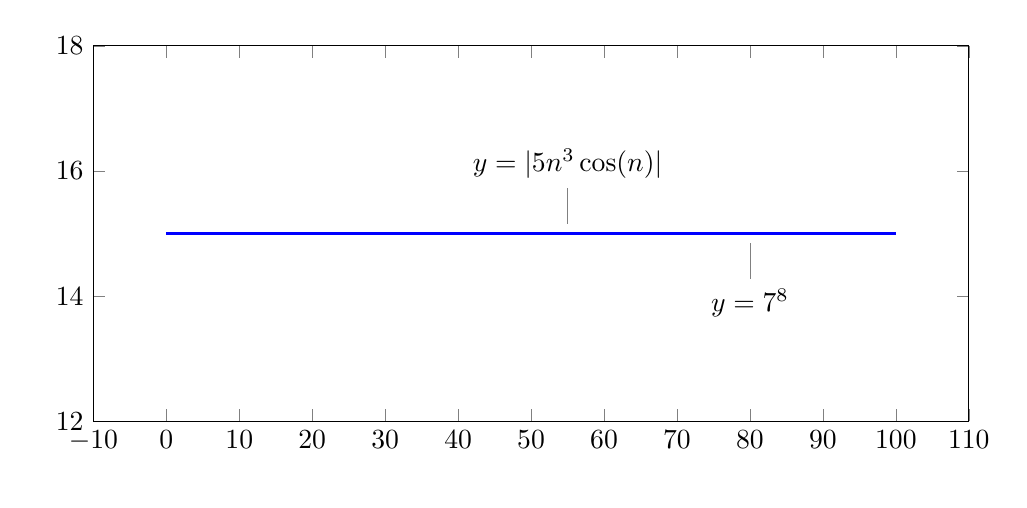
\begin{tikzpicture}[line width=1]
\begin{axis}[width=5in, height=2.5in,
             scatter/classes={a={mark=*,draw=black}},
             xlabel={\mbox{}},
             xlabel style={name=xlabel}, 
             ylabel={\mbox{}}, 
             legend style={
                at={(xlabel.south)},
                yshift=-1ex,
                anchor=north,
                legend cell align=left,
                },
        ]
]
\addplot[draw=red, line width=1] coordinates {(0.0,15)
(50.0,15)
(100.0,15)
(100.0,15)};\node[pin=above:{$y=|5n^3 \cos(n)|$}] at (axis cs:55,15) {};\addplot[draw=blue, line width=1] coordinates {(0.0,15)
(50.0,15)
(100.0,15)
(100.0,15)};\node[pin=below:{$y=7^8$}] at (axis cs:80,15) {};
\end{axis}\end{tikzpicture}\end{center}

The two graphs are the same.
If I set $C_2 = 7^8$ and $N_2 = 0$, then for $n \geq N_2$,
\[
|f_2(n)| \leq C_2|n^0|
\]
Therefore
\[
f_2(n) = O(n^0)
\]

(d) Let $C = \max(C_0, C_1, C_2) = \max(20, 5, 7^8) = 7^8$,
$N = \max(N_0, N_1, N_2) = \max(1, 0, 0) = 1$,
$k = \max(2, 3, 0) = 3$.

%-*-latex-*-

\begin{center}
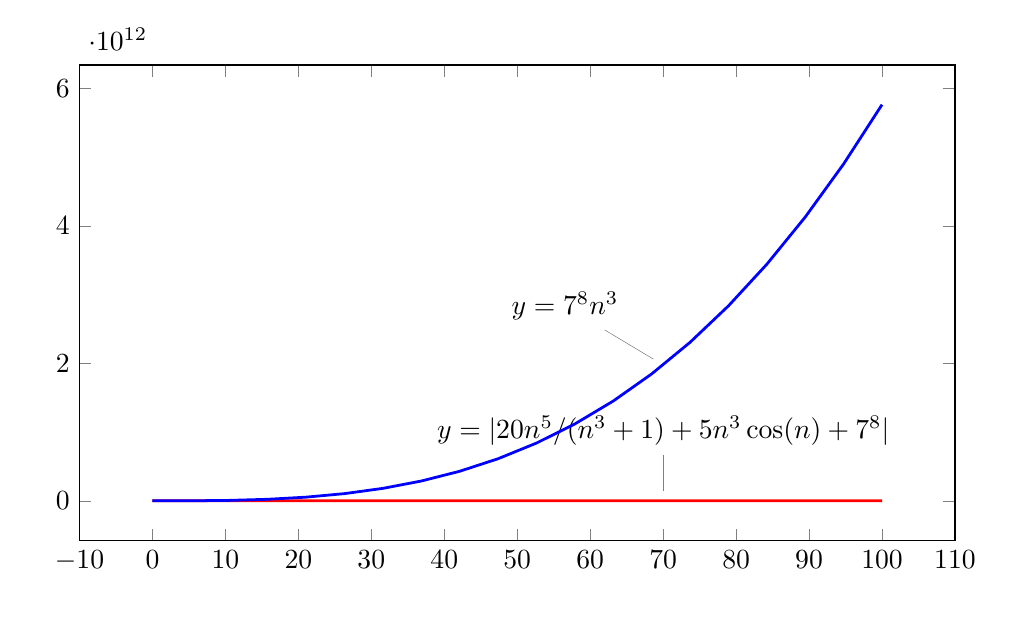
\begin{tikzpicture}[line width=1]
\begin{axis}[width=5in, height=3in,
             scatter/classes={a={mark=*,draw=black}},
             xlabel={\mbox{}},
             xlabel style={name=xlabel}, 
             ylabel={\mbox{}}, 
             legend style={
                at={(xlabel.south)},
                yshift=-1ex,
                anchor=north,
                legend cell align=left,
                },
        ]
]
\addplot[draw=red, line width=1] coordinates {(0.0,5764801.0)
(0.2506,5764801.0957)
(0.5013,5764802.1143)
(0.7519,5764805.9247)
(1.0025,5764813.7992)
(1.2531,5764824.8977)
(1.5038,5764837.0872)
(1.7544,5764848.0098)
(2.005,5764855.5726)
(2.2556,5764858.3048)
(2.5063,5764855.7689)
(2.7569,5764848.9742)
(3.0075,5764840.6923)
(3.2581,5764835.5831)
(3.5088,5764840.0649)
(3.7594,5764861.8872)
(4.01,5764909.4088)
(4.2607,5764990.6137)
(4.5113,5765111.9463)
(4.7619,5765277.0759)
(5.0125,5765485.7288)
(5.2632,5765732.7432)
(5.5138,5766007.4936)
(5.7644,5766293.8204)
(6.015,5766570.5579)
(6.2657,5766812.7075)
(6.5163,5766993.24)
(6.7669,5767085.4414)
(7.0175,5767065.6491)
(7.2682,5766916.1658)
(7.5188,5766628.0878)
(7.7694,5766203.7597)
(8.0201,5765658.5614)
(8.2707,5765021.762)
(8.5213,5764336.2227)
(8.7719,5763656.817)
(9.0226,5763047.529)
(9.2732,5762577.3164)
(9.5238,5762314.9358)
(9.7744,5762323.055)
(10.0251,5762652.071)
(10.2757,5763334.1323)
(10.5263,5764377.9028)
(10.7769,5765764.6047)
(11.0276,5767445.8259)
(11.2782,5769343.4885)
(11.5288,5771352.2321)
(11.7794,5773344.2955)
(12.0301,5775176.7832)
(12.2807,5776700.9931)
(12.5313,5777773.283)
(12.782,5778266.7746)
(13.0326,5778083.0523)
(13.2832,5777162.9364)
(13.5338,5775495.3854)
(13.7845,5773123.6444)
(14.0351,5770147.8835)
(14.2857,5766723.7749)
(14.5363,5763056.7207)
(14.787,5759391.7529)
(15.0376,5755999.4638)
(15.2882,5753158.6582)
(15.5388,5751136.735)
(15.7895,5750169.0613)
(16.0401,5750438.7942)
(16.2907,5752058.6906)
(16.5414,5755056.4308)
(16.792,5759364.8452)
(17.0426,5764818.1831)
(17.2932,5771155.2074)
(17.5439,5778029.4593)
(17.7945,5785026.5322)
(18.0451,5791687.6718)
(18.2957,5797538.4986)
(18.5464,5802121.1832)
(18.797,5805028.0285)
(19.0476,5805934.1529)
(19.2982,5804626.8647)
(19.5489,5801029.3762)
(19.7995,5795216.7441)
(20.0501,5787422.3263)
(20.3008,5778033.6031)
(20.5514,5767576.889)
(20.802,5756691.2192)
(21.0526,5746092.484)
(21.3033,5736529.6516)
(21.5539,5728735.6013)
(21.8045,5723375.6414)
(22.0551,5720997.1536)
(22.3058,5721983.951)
(22.5564,5726518.8415)
(22.807,5734557.5391)
(23.0576,5745816.4691)
(23.3083,5759776.2106)
(23.5589,5775701.3329)
(23.8095,5792676.2945)
(24.0602,5809655.9334)
(24.3108,5825527.9789)
(24.5614,5839184.028)
(24.812,5849594.6296)
(25.0627,5855883.5804)
(25.3133,5857396.3038)
(25.5639,5853757.2884)
(25.8145,5844912.0283)
(26.0652,5831149.7088)
(26.3158,5813103.9863)
(26.5664,5791730.5622)
(26.817,5768261.7639)
(27.0677,5744139.9261)
(27.3183,5720932.9083)
(27.5689,5700236.483)
(27.8195,5683569.4739)
(28.0702,5672268.3325)
(28.3208,5667388.2294)
(28.5714,5669617.6721)
(28.8221,5679213.1044)
(29.0727,5695958.9286)
(29.3233,5719156.9527)
(29.5739,5747647.4823)
(29.8246,5779862.2536)
(30.0752,5813907.2751)
(30.3258,5847671.5309)
(30.5764,5878955.5662)
(30.8271,5905612.3464)
(31.0777,5925691.588)
(31.3283,5937578.1066)
(31.5789,5940114.6729)
(31.8296,5932700.4561)
(32.0802,5915357.3467)
(32.3308,5888758.2359)
(32.5815,5854213.5937)
(32.8321,5813615.3032)
(33.0827,5769339.506)
(33.3333,5724113.0273)
(33.584,5680850.5751)
(33.8346,5642472.175)
(34.0852,5611712.0349)
(34.3358,5590931.0955)
(34.5865,5581945.8152)
(34.8371,5585885.2057)
(35.0877,5603086.7817)
(35.3383,5633039.9669)
(35.589,5674382.7208)
(35.8396,5724953.8765)
(36.0902,5781900.0972)
(36.3409,5841832.7097)
(36.5915,5901026.1788)
(36.8421,5955646.9052)
(37.0927,6001998.5607)
(37.3434,6036768.53)
(37.594,6057259.3282)
(37.8446,6061589.2097)
(38.0952,6048847.5785)
(38.3459,6019193.2171)
(38.5965,5973886.6348)
(38.8471,5915251.8289)
(39.0977,5846567.2014)
(39.3484,5771890.0168)
(39.599,5695823.313)
(39.8496,5623238.2934)
(40.1003,5558968.6365)
(40.3509,5507495.6222)
(40.6015,5472644.2799)
(40.8521,5457310.7955)
(41.1028,5463240.1171)
(41.3534,5490870.1139)
(41.604,5539254.8871)
(41.8546,5606075.1214)
(42.1053,5687737.9604)
(42.3559,5779563.138)
(42.6065,5876046.3477)
(42.8571,5971185.4757)
(43.1078,6058850.7137)
(43.3584,6133176.0424)
(43.609,6188947.3977)
(43.8596,6221962.1918)
(44.1103,6229335.8499)
(44.3609,6209733.6405)
(44.6115,6163510.1952)
(44.8622,6092744.5198)
(45.1128,6001164.6869)
(45.3634,5893963.3702)
(45.614,5777512.5194)
(45.8647,5658992.2969)
(46.1153,5545955.4674)
(46.3659,5445853.3183)
(46.6165,5365552.5368)
(46.8672,5310874.0119)
(47.1178,5286184.1119)
(47.3684,5294066.5652)
(47.619,5335098.7489)
(47.8697,5407750.1818)
(48.1203,5508413.6654)
(48.3709,5631571.2533)
(48.6216,5770088.5708)
(48.8722,5915622.4945)
(49.1228,6059119.4013)
(49.3734,6191374.635)
(49.6241,6303618.9763)
(49.8747,6388095.1102)
(50.1253,6438586.6074)
(50.3759,6450863.869)
(50.6266,6423015.7786)
(50.8772,6355642.253)
(51.1278,6251891.1222)
(51.3784,6117332.3322)
(51.6291,5959672.7526)
(51.8797,5788325.2562)
(52.1303,5613855.5389)
(52.381,5447338.7146)
(52.6316,5299664.4686)
(52.8822,5180833.9877)
(53.1328,5099293.6534)
(53.3835,5061349.4035)
(53.6341,5070701.7173)
(53.8847,5128134.5407)
(54.1353,5231382.4918)
(54.386,5375189.8945)
(54.6366,5551563.2129)
(54.8872,5750206.0589)
(55.1378,5959113.8984)
(55.3885,6165294.6738)
(55.6391,6355572.5408)
(55.8897,6517425.3997)
(56.1404,6639803.3906)
(56.391,6713875.318)
(56.6416,6733653.1699)
(56.8922,6696451.3988)
(57.1429,6603147.0871)
(57.3935,6458219.0133)
(57.6441,6269557.2488)
(57.8947,6048049.4345)
(58.1454,5806964.3808)
(58.396,5561167.1871)
(58.6466,5326211.776)
(58.8972,5117365.7957)
(59.1479,4948628.5974)
(59.3985,4831805.0005)
(59.6491,4775695.5811)
(59.8997,4785458.2977)
(60.1504,4862186.67)
(60.401,5002736.9877)
(60.6516,5199821.8812)
(60.9023,5442370.9519)
(61.1529,5716142.0618)
(61.4035,6004550.422)
(61.6541,6289667.8478)
(61.9048,6553332.4837)
(62.1554,6778300.7567)
(62.406,6949368.9458)
(62.6566,7054391.9353)
(62.9073,7085131.5399)
(63.1579,7037876.0675)
(63.4085,6913786.0182)
(63.6591,6718937.2616)
(63.9098,6464051.7016)
(64.1604,6163925.1915)
(64.411,5836582.0544)
(64.6617,5502203.7408)
(64.9123,5181894.7133)
(65.1629,4896360.5285)
(65.4135,4664580.4526)
(65.6642,4502559.2035)
(65.9148,4422239.3169)
(66.1654,4430647.2486)
(66.416,4529333.0696)
(66.6667,4714146.2274)
(66.9173,4975369.3464)
(67.1679,5298209.6764)
(67.4185,5663624.9463)
(67.6692,6049438.507)
(67.9198,6431679.1647)
(68.1704,6786065.3156)
(68.4211,7089541.992)
(68.6717,7321774.0227)
(68.9223,7466499.1672)
(69.1729,7512651.9017)
(69.4236,7455181.2006)
(69.6742,7295503.5035)
(69.9248,7041554.0431)
(70.1754,6707424.5261)
(70.4261,6312601.2781)
(70.6767,5880843.7448)
(70.9273,5438767.0299)
(71.1779,5014212.3831)
(71.4286,4634504.8604)
(71.6792,4324706.6817)
(71.9298,4105977.386)
(72.1805,3994147.4249)
(72.4311,3998600.4818)
(72.6817,4121542.1325)
(72.9323,4357709.4721)
(73.183,4694549.3826)
(73.4336,5112863.8392)
(73.6842,5587890.8752)
(73.9348,6090761.4326)
(74.1855,6590247.1647)
(74.4361,7054693.9866)
(74.6867,7454022.2015)
(74.9373,7761667.3638)
(75.188,7956337.2612)
(75.4386,8023469.5844)
(75.6892,7956291.5742)
(75.9398,7756406.286)
(76.1905,7433858.7239)
(76.4411,7006667.2576)
(76.6917,6499839.4669)
(76.9424,5943924.7342)
(77.193,5373186.4068)
(77.4436,4823502.1786)
(77.6942,4330120.7592)
(77.9449,3925414.5392)
(78.1955,3636770.9425)
(78.4461,3484759.1096)
(78.6967,3481693.6964)
(78.9474,3630694.6812)
(79.198,3925312.4418)
(79.4486,4349752.7676)
(79.6992,4879698.9965)
(79.9499,5483690.4708)
(80.2005,6124980.3706)
(80.4511,6763764.0669)
(80.7018,7359643.5373)
(80.9524,7874175.8571)
(81.203,8273345.5833)
(81.4536,8529802.6887)
(81.7043,8624719.6399)
(81.9549,8549142.6819)
(82.2055,8304742.1999)
(82.4561,7903903.4317)
(82.7068,7369139.615)
(82.9574,6731852.347)
(83.208,6030505.8347)
(83.4586,5308320.1471)
(83.7093,4610621.0288)
(83.9599,3982008.1314)
(84.2105,3463517.9783)
(84.4612,3089961.4905)
(84.7118,2887608.0591)
(84.9624,2872369.2396)
(85.213,3048606.175)
(85.4637,3408647.4891)
(85.7143,3933060.8509)
(85.9649,4591674.3577)
(86.2155,5345296.2475)
(86.4662,6148036.2374)
(86.7168,6950091.9255)
(86.9674,7700831.7973)
(87.218,8351984.6253)
(87.4687,8860734.9851)
(87.7193,9192527.0915)
(87.9699,9323394.2268)
(88.2206,9241657.9629)
(88.4712,8948878.6567)
(88.7218,8459984.137)
(88.9724,7802554.3534)
(89.2231,7015292.8893)
(89.4737,6145768.3158)
(89.7243,5247556.0564)
(89.9749,4376951.6467)
(90.2256,3589456.324)
(90.4762,2936253.6933)
(90.7268,2460900.4564)
(90.9774,2196444.3577)
(91.2281,2163158.9845)
(91.4787,2367049.1326)
(91.7293,2799234.1721)
(91.9799,3436262.9984)
(92.2306,4241356.0174)
(92.4812,5166510.807)
(92.7318,6155352.344)
(92.9825,7146559.568)
(93.2331,8077660.8007)
(93.4837,8888963.793)
(93.7343,9527373.8426)
(93.985,9949856.517)
(94.2356,10126320.09)
(94.4862,10041725.9234)
(94.7368,9697280.8322)
(94.9875,9110621.2616)
(95.2381,8314961.4985)
(95.4887,7357243.2887)
(95.7393,6295388.0488)
(95.99,5194811.2789)
(96.2406,4124408.0168)
(96.4912,3152254.9509)
(96.7419,2341296.6123)
(96.9925,1745288.2731)
(97.2431,1405256.1949)
(97.4937,1346707.2028)
(97.7444,1577775.7461)
(97.995,2088440.2049)
(98.2456,2850874.5767)
(98.4962,3820930.8547)
(98.7469,4940675.7897)
(98.9975,6141837.841)
(99.2481,7349960.3203)
(99.4987,8489008.9313)
(99.7494,9486149.3197)
(100.0,10276395.1614)};\node[pin=above:{$y=|20n^5 /(n^3 + 1) + 5n^3 \cos(n) + 7^8|$}] at (axis cs:70,6948943.147579552) {};\addplot[draw=blue, line width=1] coordinates {(0.0,0.0)
(5.2632,840472517.8597)
(10.5263,6723780142.878)
(15.7895,22692757982.2132)
(21.0526,53790241143.0238)
(26.3158,105059064732.4683)
(31.5789,181542063857.7052)
(36.8421,288282073625.8931)
(42.1053,430321929144.1902)
(47.3684,612704465519.7552)
(52.6316,840472517859.7465)
(57.8947,1118668921271.3225)
(63.1579,1452336510861.6418)
(68.4211,1846518121737.8638)
(73.6842,2306256589007.146)
(78.9474,2836594747776.6465)
(84.2105,3442575433153.525)
(89.4737,4129241480244.9395)
(94.7368,4901635724158.049)
(100.0,5764801000000.0)};\node[pin=above left:{$y=7^8 n^3$}] at (axis cs:70,1977326743000) {};
\end{axis}\end{tikzpicture}\end{center}

No. $f(n)$ is not flat.
It appears to be flat only because $7^8n^3$ is climbing too fast.
Here's the plot of $f(n)$ without $7^8n^3$

\begin{center}
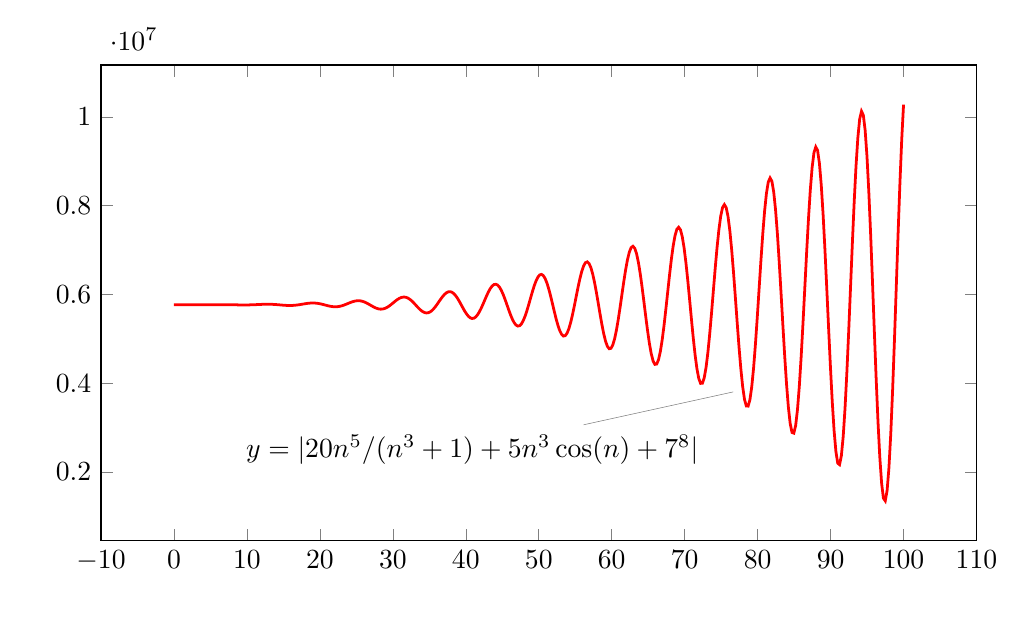
\begin{tikzpicture}[line width=1]
\begin{axis}[width=5in, height=3in,
             scatter/classes={a={mark=*,draw=black}},
             xlabel={\mbox{}},
             xlabel style={name=xlabel}, 
             ylabel={\mbox{}}, 
             legend style={
                at={(xlabel.south)},
                yshift=-1ex,
                anchor=north,
                legend cell align=left,
                },
        ]
]
\addplot[draw=red, line width=1] coordinates {(0.0,5764801.0)
(0.2506,5764801.0957)
(0.5013,5764802.1143)
(0.7519,5764805.9247)
(1.0025,5764813.7992)
(1.2531,5764824.8977)
(1.5038,5764837.0872)
(1.7544,5764848.0098)
(2.005,5764855.5726)
(2.2556,5764858.3048)
(2.5063,5764855.7689)
(2.7569,5764848.9742)
(3.0075,5764840.6923)
(3.2581,5764835.5831)
(3.5088,5764840.0649)
(3.7594,5764861.8872)
(4.01,5764909.4088)
(4.2607,5764990.6137)
(4.5113,5765111.9463)
(4.7619,5765277.0759)
(5.0125,5765485.7288)
(5.2632,5765732.7432)
(5.5138,5766007.4936)
(5.7644,5766293.8204)
(6.015,5766570.5579)
(6.2657,5766812.7075)
(6.5163,5766993.24)
(6.7669,5767085.4414)
(7.0175,5767065.6491)
(7.2682,5766916.1658)
(7.5188,5766628.0878)
(7.7694,5766203.7597)
(8.0201,5765658.5614)
(8.2707,5765021.762)
(8.5213,5764336.2227)
(8.7719,5763656.817)
(9.0226,5763047.529)
(9.2732,5762577.3164)
(9.5238,5762314.9358)
(9.7744,5762323.055)
(10.0251,5762652.071)
(10.2757,5763334.1323)
(10.5263,5764377.9028)
(10.7769,5765764.6047)
(11.0276,5767445.8259)
(11.2782,5769343.4885)
(11.5288,5771352.2321)
(11.7794,5773344.2955)
(12.0301,5775176.7832)
(12.2807,5776700.9931)
(12.5313,5777773.283)
(12.782,5778266.7746)
(13.0326,5778083.0523)
(13.2832,5777162.9364)
(13.5338,5775495.3854)
(13.7845,5773123.6444)
(14.0351,5770147.8835)
(14.2857,5766723.7749)
(14.5363,5763056.7207)
(14.787,5759391.7529)
(15.0376,5755999.4638)
(15.2882,5753158.6582)
(15.5388,5751136.735)
(15.7895,5750169.0613)
(16.0401,5750438.7942)
(16.2907,5752058.6906)
(16.5414,5755056.4308)
(16.792,5759364.8452)
(17.0426,5764818.1831)
(17.2932,5771155.2074)
(17.5439,5778029.4593)
(17.7945,5785026.5322)
(18.0451,5791687.6718)
(18.2957,5797538.4986)
(18.5464,5802121.1832)
(18.797,5805028.0285)
(19.0476,5805934.1529)
(19.2982,5804626.8647)
(19.5489,5801029.3762)
(19.7995,5795216.7441)
(20.0501,5787422.3263)
(20.3008,5778033.6031)
(20.5514,5767576.889)
(20.802,5756691.2192)
(21.0526,5746092.484)
(21.3033,5736529.6516)
(21.5539,5728735.6013)
(21.8045,5723375.6414)
(22.0551,5720997.1536)
(22.3058,5721983.951)
(22.5564,5726518.8415)
(22.807,5734557.5391)
(23.0576,5745816.4691)
(23.3083,5759776.2106)
(23.5589,5775701.3329)
(23.8095,5792676.2945)
(24.0602,5809655.9334)
(24.3108,5825527.9789)
(24.5614,5839184.028)
(24.812,5849594.6296)
(25.0627,5855883.5804)
(25.3133,5857396.3038)
(25.5639,5853757.2884)
(25.8145,5844912.0283)
(26.0652,5831149.7088)
(26.3158,5813103.9863)
(26.5664,5791730.5622)
(26.817,5768261.7639)
(27.0677,5744139.9261)
(27.3183,5720932.9083)
(27.5689,5700236.483)
(27.8195,5683569.4739)
(28.0702,5672268.3325)
(28.3208,5667388.2294)
(28.5714,5669617.6721)
(28.8221,5679213.1044)
(29.0727,5695958.9286)
(29.3233,5719156.9527)
(29.5739,5747647.4823)
(29.8246,5779862.2536)
(30.0752,5813907.2751)
(30.3258,5847671.5309)
(30.5764,5878955.5662)
(30.8271,5905612.3464)
(31.0777,5925691.588)
(31.3283,5937578.1066)
(31.5789,5940114.6729)
(31.8296,5932700.4561)
(32.0802,5915357.3467)
(32.3308,5888758.2359)
(32.5815,5854213.5937)
(32.8321,5813615.3032)
(33.0827,5769339.506)
(33.3333,5724113.0273)
(33.584,5680850.5751)
(33.8346,5642472.175)
(34.0852,5611712.0349)
(34.3358,5590931.0955)
(34.5865,5581945.8152)
(34.8371,5585885.2057)
(35.0877,5603086.7817)
(35.3383,5633039.9669)
(35.589,5674382.7208)
(35.8396,5724953.8765)
(36.0902,5781900.0972)
(36.3409,5841832.7097)
(36.5915,5901026.1788)
(36.8421,5955646.9052)
(37.0927,6001998.5607)
(37.3434,6036768.53)
(37.594,6057259.3282)
(37.8446,6061589.2097)
(38.0952,6048847.5785)
(38.3459,6019193.2171)
(38.5965,5973886.6348)
(38.8471,5915251.8289)
(39.0977,5846567.2014)
(39.3484,5771890.0168)
(39.599,5695823.313)
(39.8496,5623238.2934)
(40.1003,5558968.6365)
(40.3509,5507495.6222)
(40.6015,5472644.2799)
(40.8521,5457310.7955)
(41.1028,5463240.1171)
(41.3534,5490870.1139)
(41.604,5539254.8871)
(41.8546,5606075.1214)
(42.1053,5687737.9604)
(42.3559,5779563.138)
(42.6065,5876046.3477)
(42.8571,5971185.4757)
(43.1078,6058850.7137)
(43.3584,6133176.0424)
(43.609,6188947.3977)
(43.8596,6221962.1918)
(44.1103,6229335.8499)
(44.3609,6209733.6405)
(44.6115,6163510.1952)
(44.8622,6092744.5198)
(45.1128,6001164.6869)
(45.3634,5893963.3702)
(45.614,5777512.5194)
(45.8647,5658992.2969)
(46.1153,5545955.4674)
(46.3659,5445853.3183)
(46.6165,5365552.5368)
(46.8672,5310874.0119)
(47.1178,5286184.1119)
(47.3684,5294066.5652)
(47.619,5335098.7489)
(47.8697,5407750.1818)
(48.1203,5508413.6654)
(48.3709,5631571.2533)
(48.6216,5770088.5708)
(48.8722,5915622.4945)
(49.1228,6059119.4013)
(49.3734,6191374.635)
(49.6241,6303618.9763)
(49.8747,6388095.1102)
(50.1253,6438586.6074)
(50.3759,6450863.869)
(50.6266,6423015.7786)
(50.8772,6355642.253)
(51.1278,6251891.1222)
(51.3784,6117332.3322)
(51.6291,5959672.7526)
(51.8797,5788325.2562)
(52.1303,5613855.5389)
(52.381,5447338.7146)
(52.6316,5299664.4686)
(52.8822,5180833.9877)
(53.1328,5099293.6534)
(53.3835,5061349.4035)
(53.6341,5070701.7173)
(53.8847,5128134.5407)
(54.1353,5231382.4918)
(54.386,5375189.8945)
(54.6366,5551563.2129)
(54.8872,5750206.0589)
(55.1378,5959113.8984)
(55.3885,6165294.6738)
(55.6391,6355572.5408)
(55.8897,6517425.3997)
(56.1404,6639803.3906)
(56.391,6713875.318)
(56.6416,6733653.1699)
(56.8922,6696451.3988)
(57.1429,6603147.0871)
(57.3935,6458219.0133)
(57.6441,6269557.2488)
(57.8947,6048049.4345)
(58.1454,5806964.3808)
(58.396,5561167.1871)
(58.6466,5326211.776)
(58.8972,5117365.7957)
(59.1479,4948628.5974)
(59.3985,4831805.0005)
(59.6491,4775695.5811)
(59.8997,4785458.2977)
(60.1504,4862186.67)
(60.401,5002736.9877)
(60.6516,5199821.8812)
(60.9023,5442370.9519)
(61.1529,5716142.0618)
(61.4035,6004550.422)
(61.6541,6289667.8478)
(61.9048,6553332.4837)
(62.1554,6778300.7567)
(62.406,6949368.9458)
(62.6566,7054391.9353)
(62.9073,7085131.5399)
(63.1579,7037876.0675)
(63.4085,6913786.0182)
(63.6591,6718937.2616)
(63.9098,6464051.7016)
(64.1604,6163925.1915)
(64.411,5836582.0544)
(64.6617,5502203.7408)
(64.9123,5181894.7133)
(65.1629,4896360.5285)
(65.4135,4664580.4526)
(65.6642,4502559.2035)
(65.9148,4422239.3169)
(66.1654,4430647.2486)
(66.416,4529333.0696)
(66.6667,4714146.2274)
(66.9173,4975369.3464)
(67.1679,5298209.6764)
(67.4185,5663624.9463)
(67.6692,6049438.507)
(67.9198,6431679.1647)
(68.1704,6786065.3156)
(68.4211,7089541.992)
(68.6717,7321774.0227)
(68.9223,7466499.1672)
(69.1729,7512651.9017)
(69.4236,7455181.2006)
(69.6742,7295503.5035)
(69.9248,7041554.0431)
(70.1754,6707424.5261)
(70.4261,6312601.2781)
(70.6767,5880843.7448)
(70.9273,5438767.0299)
(71.1779,5014212.3831)
(71.4286,4634504.8604)
(71.6792,4324706.6817)
(71.9298,4105977.386)
(72.1805,3994147.4249)
(72.4311,3998600.4818)
(72.6817,4121542.1325)
(72.9323,4357709.4721)
(73.183,4694549.3826)
(73.4336,5112863.8392)
(73.6842,5587890.8752)
(73.9348,6090761.4326)
(74.1855,6590247.1647)
(74.4361,7054693.9866)
(74.6867,7454022.2015)
(74.9373,7761667.3638)
(75.188,7956337.2612)
(75.4386,8023469.5844)
(75.6892,7956291.5742)
(75.9398,7756406.286)
(76.1905,7433858.7239)
(76.4411,7006667.2576)
(76.6917,6499839.4669)
(76.9424,5943924.7342)
(77.193,5373186.4068)
(77.4436,4823502.1786)
(77.6942,4330120.7592)
(77.9449,3925414.5392)
(78.1955,3636770.9425)
(78.4461,3484759.1096)
(78.6967,3481693.6964)
(78.9474,3630694.6812)
(79.198,3925312.4418)
(79.4486,4349752.7676)
(79.6992,4879698.9965)
(79.9499,5483690.4708)
(80.2005,6124980.3706)
(80.4511,6763764.0669)
(80.7018,7359643.5373)
(80.9524,7874175.8571)
(81.203,8273345.5833)
(81.4536,8529802.6887)
(81.7043,8624719.6399)
(81.9549,8549142.6819)
(82.2055,8304742.1999)
(82.4561,7903903.4317)
(82.7068,7369139.615)
(82.9574,6731852.347)
(83.208,6030505.8347)
(83.4586,5308320.1471)
(83.7093,4610621.0288)
(83.9599,3982008.1314)
(84.2105,3463517.9783)
(84.4612,3089961.4905)
(84.7118,2887608.0591)
(84.9624,2872369.2396)
(85.213,3048606.175)
(85.4637,3408647.4891)
(85.7143,3933060.8509)
(85.9649,4591674.3577)
(86.2155,5345296.2475)
(86.4662,6148036.2374)
(86.7168,6950091.9255)
(86.9674,7700831.7973)
(87.218,8351984.6253)
(87.4687,8860734.9851)
(87.7193,9192527.0915)
(87.9699,9323394.2268)
(88.2206,9241657.9629)
(88.4712,8948878.6567)
(88.7218,8459984.137)
(88.9724,7802554.3534)
(89.2231,7015292.8893)
(89.4737,6145768.3158)
(89.7243,5247556.0564)
(89.9749,4376951.6467)
(90.2256,3589456.324)
(90.4762,2936253.6933)
(90.7268,2460900.4564)
(90.9774,2196444.3577)
(91.2281,2163158.9845)
(91.4787,2367049.1326)
(91.7293,2799234.1721)
(91.9799,3436262.9984)
(92.2306,4241356.0174)
(92.4812,5166510.807)
(92.7318,6155352.344)
(92.9825,7146559.568)
(93.2331,8077660.8007)
(93.4837,8888963.793)
(93.7343,9527373.8426)
(93.985,9949856.517)
(94.2356,10126320.09)
(94.4862,10041725.9234)
(94.7368,9697280.8322)
(94.9875,9110621.2616)
(95.2381,8314961.4985)
(95.4887,7357243.2887)
(95.7393,6295388.0488)
(95.99,5194811.2789)
(96.2406,4124408.0168)
(96.4912,3152254.9509)
(96.7419,2341296.6123)
(96.9925,1745288.2731)
(97.2431,1405256.1949)
(97.4937,1346707.2028)
(97.7444,1577775.7461)
(97.995,2088440.2049)
(98.2456,2850874.5767)
(98.4962,3820930.8547)
(98.7469,4940675.7897)
(98.9975,6141837.841)
(99.2481,7349960.3203)
(99.4987,8489008.9313)
(99.7494,9486149.3197)
(100.0,10276395.1614)};\node[pin=below left:{$y=|20n^5 /(n^3 + 1) + 5n^3 \cos(n) + 7^8|$}] at (axis cs:78,3851119.8760623066) {};
\end{axis}\end{tikzpicture}\end{center}


Note that the upper bound $7^8 n^3$ is not tight.
A tigher upper bound is $5n^3$.
Of course either way
\[
f(n) = O(n^3)
\]
\qed
